\documentclass[10pt,a4paper]{article}
\usepackage{ngerman}
\usepackage{sectsty, xcolor}
\usepackage{lastpage}
\usepackage{enumitem, fancyhdr, graphicx, float, makeidx, textcomp}
\usepackage[hidelinks]{hyperref}
\usepackage[hang,flushmargin]{footmisc}
\usepackage{listings}
\lstloadlanguages{SQL}
%%%
%\lstset{language=SQL}
%\begin{lstlisting}
%SELECT * FROM table WHERE id = 1;
%\end{lstlisting}
%%%
%\usepackage[backend=biber,style=numeric,sorting=none]{biblatex}
%\usepackage{biblatex}
%\addbibresource{bibliography.bib}
%\usepackage{authblk}
\makeindex

\definecolor{dunkelblau}{rgb}{0,0.4,0.6}
\subsectionfont{\color{dunkelblau}}

\title{ISF HS 2019}
\author{Victor Fernández\\Pavaskar Parameswaran}
\date{Dezember 2019}


\addtolength{\oddsidemargin}{-.875in}
\addtolength{\evensidemargin}{-.875in}
\addtolength{\textwidth}{1.75in}
\addtolength{\topmargin}{-.875in}
\addtolength{\textheight}{1.75in}

% muss nach Änderung der margin kommen!
\pagestyle{fancy}
\fancyhf{} %reset
\fancyhead[L]{HSLU}
\fancyhead[C]{ISF}
\fancyhead[R]{\thepage/\pageref{LastPage}}
\fancyfoot[L]{}
\fancyfoot[C]{}
\fancyfoot[R]{}
\renewcommand{\headrulewidth}{0.2pt} % Strich in Kopfzeile

%******
\begin{document}
\maketitle
\thispagestyle{empty}
\section*{Vorwort}Diese Zusammenfassung entstand in einer Gruppe während der Lernphase des HS 2019. Alle Fragen aus der Stoffabgrenzung tragen eine {\color{dunkelblau}blaue Farbe} und stehen als Unterkapitel. Das Dokument ist Open Source und jeder der möchte und signifikant beiträgt, darf sich als Autor anhängen. Die Source ist \underline{\href{https://github.com/vigi86/HSLU_Zusammenfassungen/tree/master/ISF_HS19}{dieses GitHub-Repo}}\footnote{https://github.com/vigi86/HSLU\_Zusammenfassungen/tree/master/ISF\_HS19}. Dies ist mein erstes \LaTeX{}-Dokument überhaupt. Nichts desto trotz wurde auf eine klare Strukturierung und Lesbarkeit des Dokumentes Wert gelegt.
\tableofcontents
\thispagestyle{empty}
\pagebreak


%%%%%%%%%%
\part{Einführung (SW~01)}
\section{Einführung}
\subsection*{Einführung in das Thema "`Management von Informationssicherheit"'}
\paragraph*{Daten, Information und Wissen}
Information ist die Verknüpfung von Daten in Form von Zahlen, Worten und Fakten zu interpretierbaren Zusammenhängen.
Durch die Vernetzung von Informationen entsteht Wissen, das zunächst personenbezogen ist.

\paragraph*{Missbrauch}Informationen müssen vor Missbrauch geschützt werden
\begin{figure}[H]
    \begin{center}
    \includegraphics[width=8cm]{images/Wissenspyramide.png}
    \caption{Wissenspyramide (Wikipedia)}
    \label{Wissenspyramide}
    \end{center}
\end{figure}

\subsection*{Motivation / Bedrohungen}
\paragraph*{Was gefährdet die Informationen?} Welche Gefährdungen/Bedrohungen gibt es?\index{Gefährdungen}\index{Bedrohungen}\index{Informationssicherheit}
\begin{itemize}[noitemsep,topsep=0pt,leftmargin=*]
    \item Nicht vorsätzliche (zufällige) Gefährdungen/Bedrohungen
    \begin{itemize}[noitemsep,topsep=0pt,leftmargin=*]
        \item Naturgewalten (Blitz, Hagel, Unwetter, Erdrutsche, Hochwasser, etc.)
        \item Ausfall von Strom oder Telekommunikation
        \item Technische Pannen, z.B. Fehler von Hard- und/oder Software
        \item Bedienerfehler / Fahrlässigkeit der Mitarbeitenden
    \end{itemize}
    \item Vorsätzliche Gefährdungen/Bedrohungen
    \begin{itemize}[noitemsep,topsep=0pt,leftmargin=*]
        \item Bösartiger Code (Viren, Würmer, Trojaner, etc.)
        \item Informationsdiebstahl
        \item Angriffe (von Skript-Kiddies bis Hacker)
        \item Wirtschaftsspionage ("`was die Konkurrenz wissen möchte"')
        \item Missbrauch der IT-Infrastruktur
    \end{itemize}
\end{itemize}


\subsection*{Grundbegriffe}\label{sec:Grundbegriffe}
\textbf{Zutritts-, Zugangs-, Zugriffskontrolle}
\begin{itemize}[noitemsep,topsep=0pt,leftmargin=*]
    \item \textbf{\textsl{Zutrittskontrolle: }}Schutz des physischen Systems (Bsp. Serverraum)\index{Zutrittskontrolle}
    \item \textbf{\textsl{Zugangskontrolle: }}Schutz des logischen Systems (Bsp. Betriebssystem)\index{Zugangskontrolle}
    \item \textbf{\textsl{Zugriffskontrolle: }}Daten-bezogen; Schutz der Operationen (Bsp. Dateisystem)\index{Zugriffskontrolle}
\end{itemize}


\subsection*{Kontrollfragen SW 01}
\paragraph*{Wie lauten die Schutzziele der Informationssicherheit? Nennen Sie konkrete Beispiele.}\index{Schutzziele}\index{Informationssicherheit}
\begin{itemize}[noitemsep,topsep=0pt,leftmargin=*]
    \item \textbf{\textsl{Verfügbarkeit:}} Zur gewünschten Zeit kann vom Benutzer auf die Daten zugegriffen werden und der Dienst funktioniert (Ausfallquote)\index{Verfügbarkeit}
    \item \textbf{\textsl{Integrität:}} Gewährleistung das Daten nicht unautorisiert oder zufällig manipuliert werden können. (Datensicherheit)\index{Integrität}
    \item \textbf{\textsl{Verbindlichkeit:}} Handlung kann eindeutig einer Person zugeordnet werden und von dieser auch nicht geleugnet werden.\index{Verbindlichkeit}
    \item \textbf{\textsl{Vertraulichkeit:}} Informationen können nicht von unautorisierten Personen, Instanzen und/oder Prozessen eingesehen werden.\index{Vertraulichkeit}
\end{itemize}
\noindent
\paragraph*{Beispiele}
\begin{itemize}[noitemsep,topsep=0pt,leftmargin=*]
    \item Daten und Informationen (Kundendaten, Rechnungen, Marketingdaten usw.) können nicht vom PC abgerufen werden.
    \item Durchgängiges Funktionieren von IT Systemen, sowie eine Vollständigkeit und Richtigkeit von Daten und Informationen. Verhindern von nicht genehmigten Veränderungen an wichtigen Informationen.
    \item Schutz vor Verrat von Informationen oder vertraulichen Daten. Mit Authentizität ist gewährleistet, dass es sich tatsächlich um eine autorisierte Person (Identiätsnachweis) handelt.
\end{itemize}
\begin{figure}[H]
    \begin{center}
    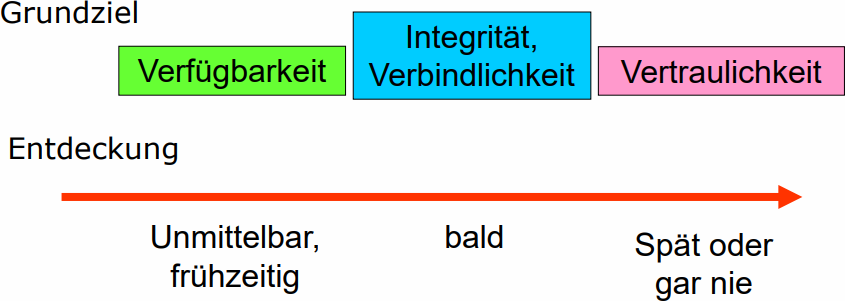
\includegraphics[width=16cm]{images/grundziel-entdeckung.png}
    \caption{Zeitpunkt der Entdeckung eines Grundziel-Verlustes}
    \label{grundziel-entdeckung}
    \end{center}
\end{figure}

\paragraph*{Erklären Sie die Zusammenhänge zwischen Risiko, Sicherheit, Eintretenshäufigkeit, Schadenshöhe, Restrisiko?}
\begin{itemize}[noitemsep,topsep=0pt,leftmargin=*]
    \item Risiko: Gefahr, Problem welches entstehen kann.\index{Risiko}
    \item Sicherheit: Schutz vor Risiko\index{Sicherheit}
    \item Eintretenshäufigkeit: Wahrscheinlichkeit, dass Risiko eintritt\index{Eintretenshäufigkeit}
    \item Restrisiko: Sicherheit deckt einen Teil des Risikos ab, jedoch nur gewisses Budget, somit bleibt Restrisiko, z.B. Erdbeben in San~Francisco oder Istanbul\index{Restrisiko}
\end{itemize}

\paragraph*{Zusammenhang}Durch Sicherheitsmassnahmen kann man die Eintretenshäufigkeit von einem Risiko mindern und somit auch den Schaden reduzieren, zusätzlich wird auch das Restrisiko kleiner oder kann sogar ausgeschlossen werden.

\paragraph*{Was ist eine Risikoanalyse? Wozu dient sie?}\index{Risikoanalyse}
\begin{enumerate}[noitemsep,topsep=0pt,leftmargin=*]
    \item Risiken zu erkennen
    \item Risiken analysieren
    \item Risikobewertung
    \item Nächster Schritt wäre das Risiko zu mindern mit den Erkenntnissen aus den ersten 3 Punkten.
    \item Massnahmen ergreifen und umsetzen.
\end{enumerate}

\paragraph*{Welche Möglichkeiten zur Behandlung (\flqq Mitigation \frqq) stehen zur Verfügung? Ordnen Sie diese in der Reihenfolge, wie man sie typischerweise anwendet. Geben Sie ein kurzes Beispiel oder eine Erläuterung}
\begin{itemize}[noitemsep,topsep=0pt,leftmargin=*]
    \item Mitigation = Verminderung
    \item Priorisieren: welches Risiko muss ich zuerst behandeln
    \item Vermindern: Massnahmen ergreifen, um Eintretenshäufigkeit und Schadensausmass zu vermindern
    \item Vermeiden: Massnahmen oder Wege einleiten um das Risiko auszuschliessen
    \item Akzeptieren: Ähnlich wie Ignorieren und das Risiko einfach hinnehmen
\end{itemize}

\paragraph*{Welche Gefährdungen und Bedrohungen kennen Sie? Gliedern Sie diese in verschiedene Kategorien.}\index{Gefährdungen}\index{Bedrohungen}
\begin{itemize}[noitemsep,topsep=0pt,leftmargin=*]
    \item Bruteforce, Phishing, DDoS, Injections, Spoofing, frustrierte Mitarbeiter, Anonymous, NSA, Naturgewalt, Hacker, Wirtschaftsspionage etc.
\end{itemize}

\subsubsection*{Stellen Sie Wissen – Information – Daten in eine Beziehung. Worauf bezieht sich die IT-Sicherheit? Was verstehen Sie unter integraler\footnote{Die Integrale Sicherheit überprüft Personen und Unternehmen mit Zugang zu vertraulichen oder geheimen Informationen, Materialien oder Anlagen. - https://www.sbis.ch} / holistischer\footnote{Ganzheitlich} Sicherheit?}\index{Wissen}\index{Information}\index{Daten}
Ziel ist das grösste Niveau der Sicherheit zu erzielen (Gesamtsystem) wichtig ist wie sich die einzelnen Sicherheitskomponenten ergänzen und zusammenspielen. (Siehe Abbildung \ref{Wissenspyramide})
\begin{itemize}[noitemsep,topsep=0pt,leftmargin=*]
    \item \textbf{Informationssicherheit:}\index{Informationssicherheit} Schutz der Information als solche, Medien unabhängig Elektronischer Datenträger
    \item \textbf{IT-Sicherheit:}\index{IT-Sicherheit} Schutz der Informationen in ICT-Systemen. (Server/Host)
    \item \textbf{Integrale Sicherheit vs. holistische Sicherheit:}\index{Integrale Sicherheit}\index{Holistische Sicherheit} Umfassende Betrachtung aller Sicherheitsaspekte einer Organisation.
\end{itemize}

\subsubsection*{Bedeutung des Managements / GL im Rahmen von AKVs}
Ohne Management-Support geht gar nichts. {\color{red}TODO: AKV???}
\begin{itemize}[noitemsep,topsep=0pt,leftmargin=*]
    \item Keine Ressourcen (Zeit und Geld)
    \item Keine Kompetenzen (Befehls-und Umsetzungsgewalt)
    \item Keine Priorität
    \item Das Management trägt die Risiken (Haftung für Mitarbeiter etc.) und entscheidet über die eingesetzten Ressourcen
    \item Häufig fehlendes Know-How der Managementetage
\end{itemize}

\paragraph*{Wie gehen Sie konkret vor, um die Informationssicherheit einzuführen?}\index{Informationssicherheit}
\begin{itemize}[noitemsep,topsep=0pt,leftmargin=*]
    \item Management ins Boot holen
    \item Prozess der Informationssicherheit etablieren (Know-How vermitteln oder zumindest das Thema greifbar machen für Management)
    \item Verantwortlichkeiten festlegen
    \item Sicherheit allumfassend betrachten
    \item Schrittweise und stetig umsetzen (kontinuierlicher Prozess)
\end{itemize}

\paragraph*{Begründen Sie, warum Informationssicherheit ein Prozess und kein Projekt sein muss.}\index{Informationssicherheit}
\begin{itemize}[noitemsep,topsep=0pt,leftmargin=*]
    \item Kontinuierliche Verbesserung der Sicherheit ein Muss
    \item Angriffe durch Hacker etc. entwickeln sich weiter, somit muss man immer auf dem neuesten Stand sein ("`up to date"' wie Dopingkontrollen im Sport)
    \item Projekt ist hingegen terminiert und irgendwann abgeschlossen
\end{itemize}

\paragraph*{Welche 3 Bereiche müssen Sie mit Ihren Massnahmen bespielen und warum?}\index{Massnahmen}
\begin{itemize}[noitemsep,topsep=0pt,leftmargin=*]
    \item Technik: kaufen und konfigurieren. Immer auf dem neuesten Stand und effizient eingesetzt.
    \item Prozesse: definieren, kontrollieren, weiterentwickeln. (Ist- und Soll-Prozess die ganze Zeit anpassen)
    \item Mitarbeiter: sensibilisieren und ausbilden. Meiner Ansicht nach auch Motivation und Loyalität fördern. (Interesse des Mitarbeiters wecken)
\end{itemize}

\paragraph*{Beschreiben Sie den Zweck von Datenschutz? Recherchieren Sie den heutigen Stand CH und die Veränderung durch die EU-DSGVO}\index{Datenschutz}
\paragraph*{TODO}

\paragraph*{Setzen Sie die Begriffe Zutritt, Zugang und Zugriff in Beziehung.}{Siehe \underline{\nameref{sec:Grundbegriffe}}, Seite \pageref{sec:Grundbegriffe}}


%%%%%%%%%%
\part{Kryptographie (SW~02-04)}
\section{Symmetrische Kryptographie}
\subsection*{Sie verstehen was Steganographie ist}
\paragraph*{Steganographie}\index{Steganographie}Verstecken von Information, z.B. in Bildern oder Audiofiles. \underline{\href{https://www.petitcolas.net/steganography/index.html}{Siehe Link}}\footnote{https://www.petitcolas.net/steganography/index.html}


\subsection*{Sie verstehen was Private-Key-Kryptographie ist, welche Arten von Sicherheit es gibt und welche Angriffsarten auf Verschlüsselung existieren}\index{Private-Key-Kryptographie}
\paragraph*{Zeichencodierung}Kodierung (\textsl{Encoding}) heisst, einen Wert mit Symbolen eines Zeichensatzes darzustellen. Beispiel:\newline %bleibt
\begin{tabular}{|ll|}
    \hline
        Dezimalsystem & 100\\
        Binärsystem & 1100100\\
        Hexadezimalsystem (`hex') & 64\\
        ASCII & hello\\
        Base64 & aGVsbG8=\\
    \hline
\end{tabular}
{\color{red}\textbf{Achtung: Kodierung $\neq$ Verschlüsselung}}

\paragraph*{Symmetrische Verschlüsselung}Bei symmetrischen Verschlüsselungsverfahren gibt es im Gegensatz zu den asymmetrischen Verfahren, \textbf{nur einen einzigen Schlüssel}. Dieser Schlüssel ist für die Verschlüsselung, als auch für die Entschlüsselung zuständig.\index{Symmetrische Kryptographie}

\paragraph*{Secret Key Verschlüsselung}Secret Key (`Symmetrische') Verschlüsselung wird zwischen zwei Parteien verwendet, welche einen \textbf{gemeinsamen Schlüssel} besitzen. Ausserdem wird sie oft verwendet, wenn der gleiche Benutzer ein Dokument verschlüsseln und zu einem späteren Zeitpunkt wieder entschlüsseln muss.\index{Secret Key}
\begin{figure}[ht]
    \begin{center}
    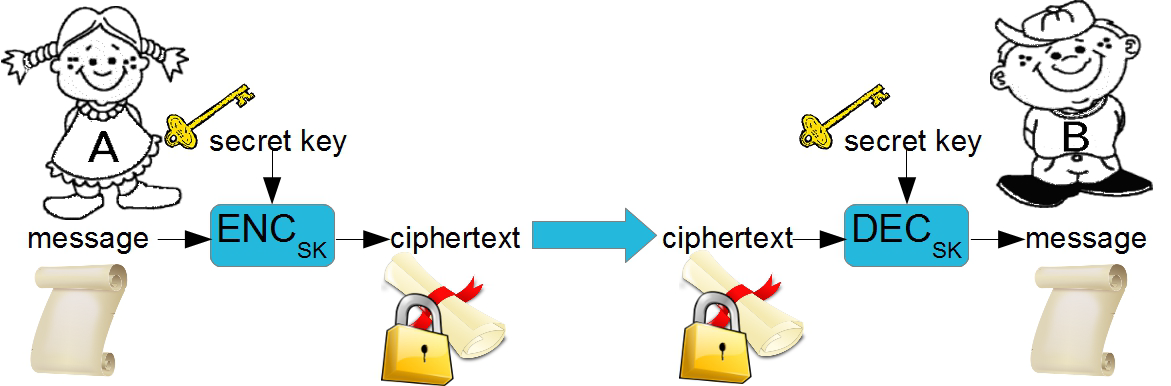
\includegraphics[width=14cm]{images/secretkey.png}
    \caption{Alice verschlüsselt, Bob entschlüsselt mit dem gemeinsamen Schlüssel}
    \label{secretkey}
    \end{center}
\end{figure}

\paragraph*{Secret Key Verschlüsselung: Algorithmen}Beispiele für symmetrische Verschlüsselung \newline
\begin{tabular}{|c|c|c|c|c|}
    \hline
    Name&Blocklänge&Schlüssellänge&Jahr&Kommentar\\
    \hline
    DES&64 Bit&56 Bit&1970&gebrochen\\
    Triple DES&64 Bit&112 Bit ($3\times56$ Bit)&  &nicht mehr empfohlen\\
    RC4&stream cipher&8-2040&1987&gebrochen\\
    IDEA&64 Bit&128 Bit&1990&nicht mehr empfohlen\\
    RC5&64 oder 128 Bit&4-256 Bit&1994&nicht mehr empfohlen\\
    Camellia&128 Bit&128, 192 oder 256 Bit&2000& \\
    Twofish&128 Bit&128, 192 oder 256 Bit&1998& \\
    AES (Rijndal)&128 Bit&128, 192 oder 256 Bit&2000& \\
    \hline
\end{tabular}

\paragraph*{Informationstheoretische Sicherheit}Das Ziel informationstheoretischer Sicherheit ist der Schutz von Daten vor unbefugtem Zugriff während der Übertragung. Im Unterschied zur Kryptographie basiert informationstheoretische Sicherheit nicht auf der Annahme, dass die Rechenleistung eines unberechtigten Empfängers nicht gross genug ist, um die Daten zu decodieren. Vielmehr garantiert informationstheoretische Sicherheit, dass ein unberechtigter Empfänger selbst bei beliebig grosser Rechenleistung nicht in der Lage ist, solcherart geschützte Nachrichten zu decodieren. Mit anderen Worten erhält ein Angreifer durch den Geheimtext keinerlei (zusätzliche) Information über den Klartext.\index{Informationstheoretische Sicherheit}%\footcite{renner2006}
 Beispielsweise ist OTP informationstheoretisch sicher. \newline %bleibt
Formal:
\begin{math}
    P(M=m) = P(M=m|C=c)
\end{math} {\color{red}Erklärung der Variablen??}

\paragraph*{Berechenmässige Sicherheit}\index{Berechenmässige Sicherheit}\label{para:Berechenmässige Sicherheit}Der sicheren Übertragung und Aufbewahrung vertraulicher Daten kommt in unserer von Information dominierten Gesellschaft immer grössere Bedeutung zu. Die heute gebräuchlichen Verfahren zur Datenverschlüsselung bieten allerdings nur beschränkte, sogenannt berechenmässige Sicherheit. Das bedeutet, dass diese prinzipiell von einem Angreifer, der über genügend Rechenleistung (zum Beispiel einen, heute noch hypothetischen, Quantencomputer) verfügt, gebrochen werden können.

\paragraph*{Kerckhoff's Prinzip}\index{Kerckhoff's Prinzip}\label{para:Kerckhoff's Prinzip}Der Angreifer kennt den Algorithmus und alle Details des Systems. Nur der Schlüssel ist geheim.

\paragraph*{Angriffsarten}Bei der Sicherheit von modernen Verschlüsselungssystemen wird zwischen den Angriffs-möglichkeiten des Angreifers unterschieden:
\begin{itemize}[noitemsep,topsep=0pt,leftmargin=*]
    \item \textbf{Ciphertext only attack:} Angreifer erhält nur den zu entschlüsselnden Geheimtext
    \begin{figure}[ht]
        \begin{center}
        \includegraphics[width=8cm]{images/coa.png}
        \caption{Nur Geheimtext}
        \label{coa}
        \end{center}
    \end{figure}\index{Ciphertext only attack}
    \item \textbf{Known plaintext attack:} Angreifer erhält zusätzlich andere Klartext-Geheimtext-Paare
    \begin{figure}[ht]
        \begin{center}
        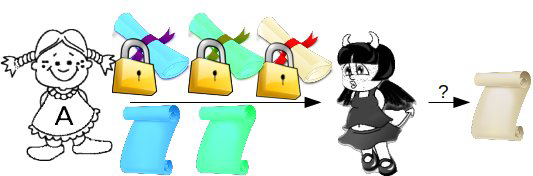
\includegraphics[width=8cm]{images/kpa.png}
        \caption{Klartext-Geheimtext-Paare}
        \label{kpa}
        \end{center}
    \end{figure}\index{Known plaintext attack}
    \item \textbf{Chosen plaintext attack:} Angreifer kann zusätzliche Klartexte wählen, zu denen er auch die Geheimtexte erhält
    \begin{figure}[ht]
        \begin{center}
        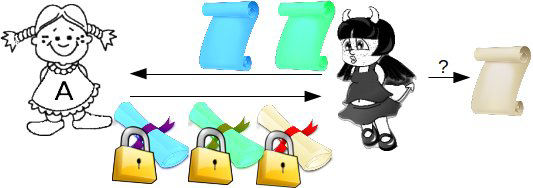
\includegraphics[width=8cm]{images/cpa.png}
        \caption{Klartexte und Geheimtexte}
        \label{cpa}
        \end{center}
    \end{figure}\index{Chosen plaintext attack}
\end{itemize}


\subsection*{Sie können "`klassische"' symmetrische Verschlüsselungverfahren wie Caesar cipher, Vigenère cipher, one-time pad anwenden und verstehen die Vor- und Nachteile bzw. Schwachstellen dieser Verfahren}\index{Klassische symmetrische Verschlüsselungsverfahren}

\paragraph*{Caesar cipher}\index{Caesar cipher}\label{para:Caesar cipher}Caesar-Verschlüsselung ist ein einfaches symmetrisches Verschlüsselungsverfahren, das auf der monographischen und monoalphabetischen Substitution basiert.\\
\textbf{Vorteil:} es ist \textbf{einfach}.\\
\textbf{Nachteil:} es ist \textbf{unsicher}, da es sehr schnell geknackt werden kann.\\
\textbf{Schwachstelle:} Die in der natürlichen Sprache ungleiche Verteilung der Buchstaben wird durch diese Art der Verschlüsselung nicht verborgen, so dass eine Häufigkeitsanalyse (Frequenzanalyse) das Wirken einer einfachen monoalphabetischen Substitution enthüllt.

\paragraph*{Caesar cipher: Vorgang}
\begin{itemize}[noitemsep,topsep=0pt,leftmargin=*]
    \item Verschiebt jeden Buchstaben des Alphabets um eine bestimmte Anzahl Stellen
    \item Soll bereits von Julius Caesar verwendet worden sein, daher der Name
    \item Der Schlüssel wird entweder als Anzahl Stellen, um die verschoben wird, oder als Buchstaben, auf den `A' verschoben wird angegeben
    \item Variante: ROT13 (Verschlüsselung = Entschlüsselung)
    \item Problem 1: Schlüssellänge (nur 26 verschiedene Schlüssel)
    \item Problem 2: Frequenzanalyse
\end{itemize}
\begin{figure}[H]
    \begin{center}
    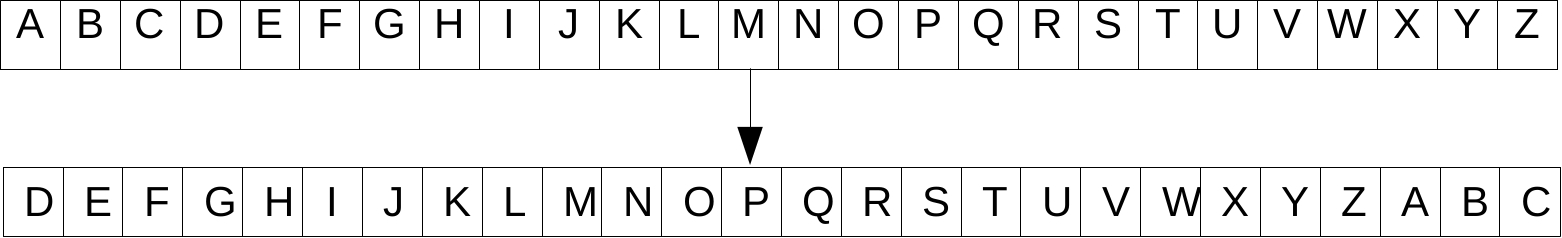
\includegraphics[width=12cm]{images/caesar.png}
    \caption{Caesar cipher mit Verschiebung um 3 Stellen}
    \label{caesar}
    \end{center}
\end{figure}

\noindent
Das folgende Diagramm zeigt die Häufigkeitsverteilung der Buchstaben in einem längeren Text in deutscher Sprache:
\begin{figure}[H]
    \begin{center}
    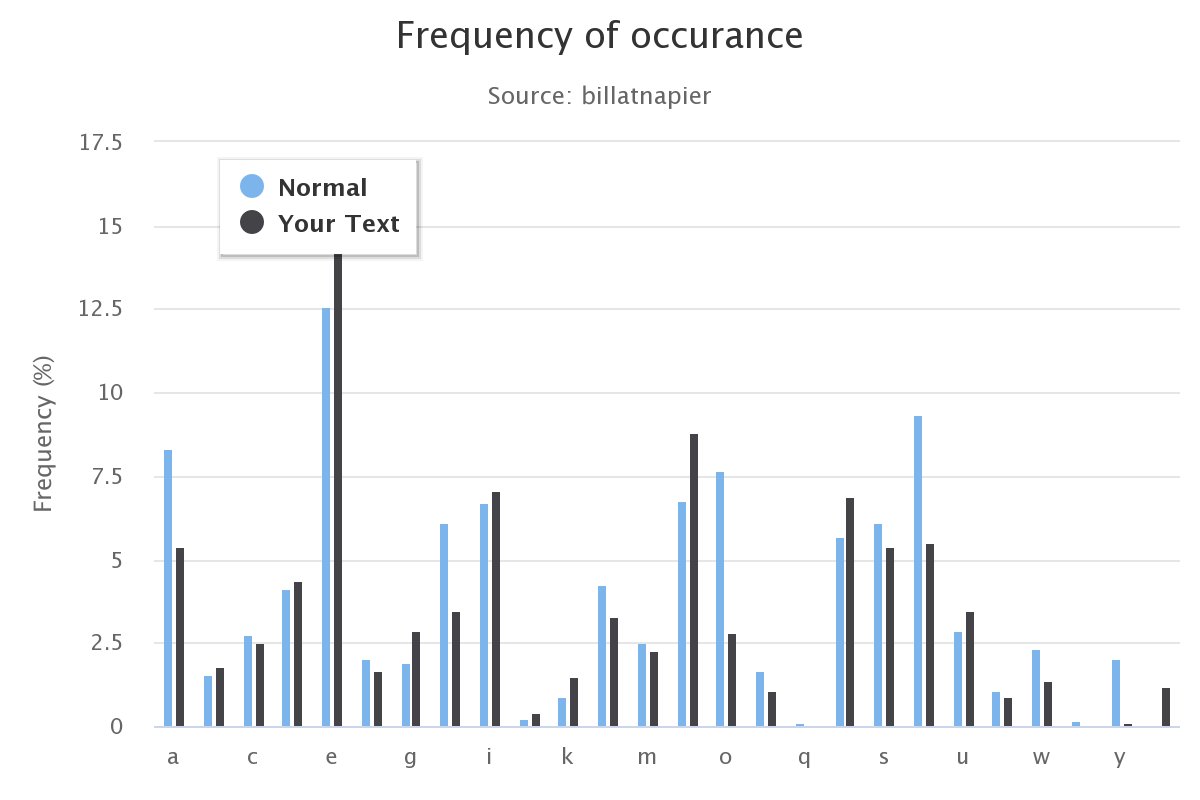
\includegraphics[width=10cm]{images/frequency0.png}
    \caption{Frequenzanalyse unchiffriert}
    \label{frequencynormal}
    \end{center}
\end{figure}

\noindent
Wie zu erwarten, ist der häufigste Buchstabe E, gefolgt von N und I, wie es im Deutschen üblicherweise der Fall ist. Wird der Text mit dem Schlüssel 10 (oder anders gesagt, mit dem Schlüsselbuchstaben J) chiffriert, erhält man einen Geheimtext, der folgende Häufigkeitsverteilung besitzt:
\begin{figure}[H]
    \begin{center}
    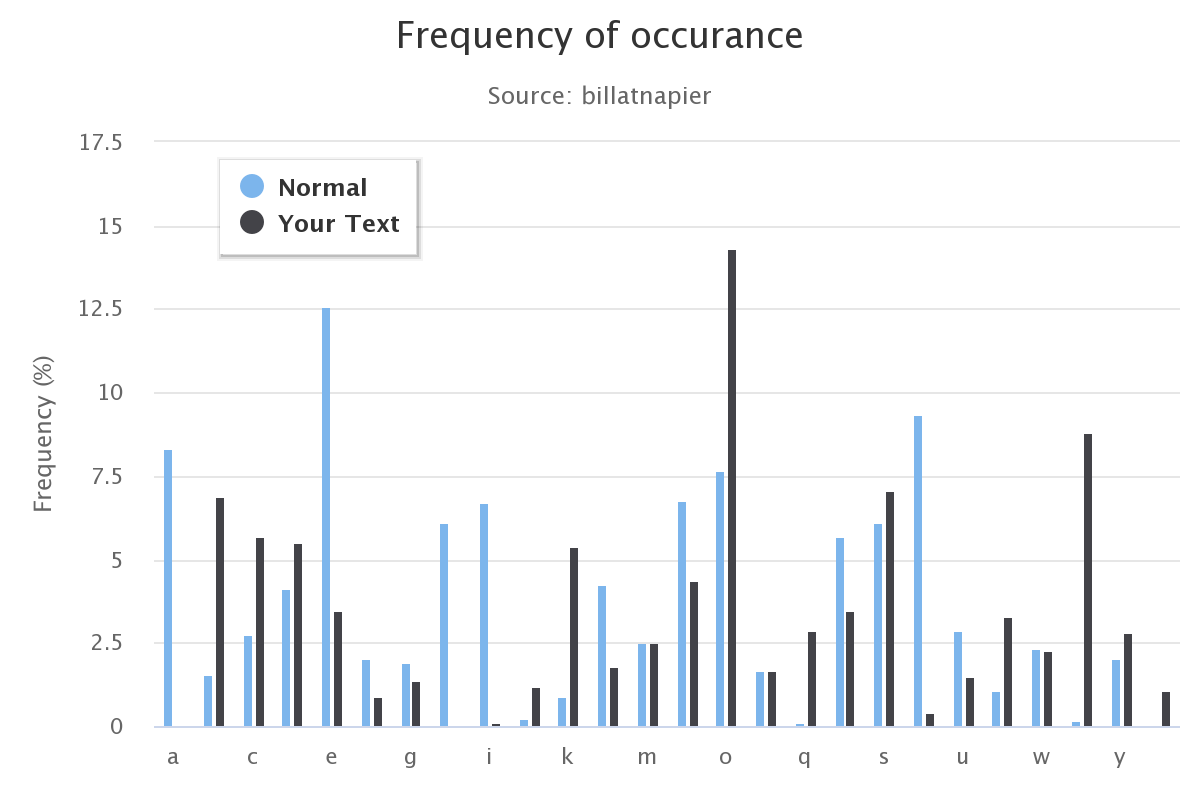
\includegraphics[width=10cm]{images/frequency1.png}
    \caption{Frequenz um 10 Stellen verschoben}
    \label{frequencycaesar}
    \end{center}
\end{figure}

\noindent
Der häufigste Buchstabe ist hier O, gefolgt von X und S. Man erkennt auf den ersten Blick die Verschiebung des deutschen "`Häufigkeitsgebirges"' um zehn Stellen nach hinten und besitzt damit den Schlüssel. Voraussetzung ist lediglich, dass man die Verteilung der Zeichen des Urtextes vorhersagen kann.

\noindent
Besitzt man diese Information nicht oder möchte man auf die Häufigkeitsanalyse verzichten, kann man auch die Tatsache ausnutzen, dass bei der Cäsar-Chiffre nur eine sehr kleine Anzahl möglicher Schlüssel in Frage kommt. Da die Größe des Schlüsselraums nur 25 beträgt, was einer "`Schlüssellänge"' von nicht einmal 5~bit entspricht, liegt nach Ausprobieren spätestens nach dem 25. Versuch der Klartext vor.

\paragraph*{Vigenère cipher}\index{Vigenère cipher}\label{para:Vigenère cipher}
\begin{itemize}[noitemsep,topsep=0pt,leftmargin=*]
    \item Schlüssel: Wort der Länge $L$
    \item Jeder Buchstabe im Text wird mit der Caesar cipher des entsprechenden Schlüsselwortes verschlüsselt
    \item Anzahl mögliche Schlüssel: $26^L$
    \item Problem: Frequenzanalyse jeder $L$'ten Stelle
\end{itemize}
\begin{figure}[H]
    \begin{center}
    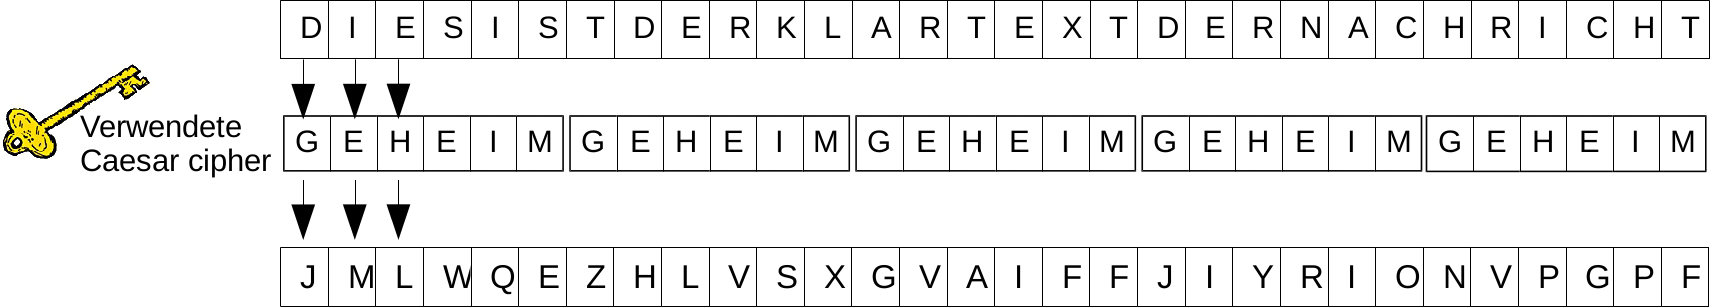
\includegraphics[width=16cm]{images/vigenere.png}
    \caption{Vigenère cipher}
    \label{vigenere}
    \end{center}
\end{figure}

\paragraph*{One-time pad}\index{One-time pad}
\begin{itemize}[noitemsep,topsep=0pt,leftmargin=*]
    \item Jede Stelle wird mit einem anderen Schlüssel verschlüsselt
    \item Darf nur 1 Mal verwendet werden!
    \item Anzahl möglicher Schlüssel = Anzahl möglicher Nachrichten
    \item Ist sicher, d.h. Geheimtext verrät keinerlei (zusätzliche) Information über den Klartext
    \item Intuitiv: Für einen bestimmten Geheimtext sind \textbf{alle} Klartexte (dieser Länge) möglich
\end{itemize}
\begin{figure}[H]
    \begin{center}
    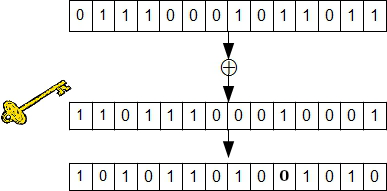
\includegraphics[width=12cm]{images/otp.png}
    \caption{Funktionsweise des OTP}
    \label{otp}
    \end{center}
\end{figure}


\subsection*{Sie wissen welche modernen Verschlüsselungsalgorithmen in der Praxis verwendet werden und was deren Eigenschaften sind}
\paragraph*{TODO}


\subsection*{Sie verstehen was eine Hashfunktion ist und welche Eigenschaften eine kryptographische Hashfunktion ausmachen, bzw. was es heisst, wenn eine Hashfunktion gebrochen ist}

\paragraph*{Hashfunktion}\index{Hashfunktion}\label{para:Hashfunktion}Eine Hashfunktion ist eine Abbildung, die eine grosse Eingabemenge (die Schlüssel) auf eine kleinere Zielmenge (die Hashwerte) abbildet. Die Eingabemenge kann Elemente unterschiedlicher Längen enthalten, die Elemente der Zielmenge haben dagegen meist eine feste Länge.
\begin{figure}[H]
    \begin{center}
    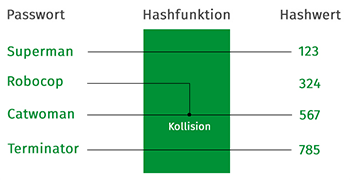
\includegraphics[width=8cm]{images/hash1.png}
    \caption{Einfaches Beispiel einer Hashfunktion}
    \label{hash1}
    \end{center}
\end{figure}

\noindent
Auf der linken Seite sehen wir 4 Passwörter von beispielsweise 4 Mitarbeitern eines Unternehmens. Die Hashfunktion  wandelt nun diese Passwörter in eine Zeichenfolge (dem Hashwert) mit einer festen Länge (hier 3 Zeichen) um. Für das Passwort "`Superman"' bekommt man den Hashwert 123, dem Passwort "`Robocop"' wird de Hashwert 567 zugeordnet, genauso wie dem Passwort "`Catwoman"' und "`Terminator"' bekommt 785.
Hashfunktionen reduzieren zunächst nur Zeichen beliebiger Länge (unterschiedliche Passwörter) auf Zeichen fester Länge (im Beispiel 3 Zeichen). Sie werden also in eine kleine, kompakte Form gebracht.

\paragraph*{Zusatzinfo zum Hashwert}Der Hashwert ist das Ergebnis, das mittels einer Hashfunktion berechnet wurde. Man definiert eine feste Länge, wie lang ein Hashwert immer sein darf. Oft wird der Hashwert als eine hexadezimale Zeichenkette codiert, d.h. der Hashwert besteht aus einer Kombination von Zahlen und Buchstaben zwischen 0 und 9 sowie A bis F (als Ersatz für die Zahlen 10 bis 15). Ein Hashwert aus 10 hexadezimalen Zeichen könnte so aussehen: "`3d180ab86e"'.

\paragraph*{Eigenschaft einer Hashfunktion}
\begin{itemize}[noitemsep,topsep=0pt,leftmargin=*]
    \item Einwegfunktion: Aus dem Hashwert darf nicht der originale Inhalt erzeugt werden können. In unserem Beispiel darf es nicht möglich sein, aus dem Hashwert "`123"' den Ursprungstext "`Superman"' zu erzeugen.
    \item Kollisionssicherheit: Den unterschiedlichen Texten darf nicht derselbe Hashwert zugeordnet sein. Ist diese Voraussetzung erfüllt, so spricht man auch von \textbf{kryptographischen Hashfunktionen}. In unserem Beispiel liegt eine Kollision vor, da die Passwörter "`Robocop"' und "`Catwoman"' denselben Hashwert haben. Damit ist die Hashfunktion im Bild nicht kollisionssicher und es handelt sich nicht um eine kryptografische Hashfunktion.
    \item Schnelligkeit: Das Verfahren zu Berechnung des Hashwertes muss schnell sein.
\end{itemize}

\paragraph*{Algorithmen für Passwortspeicherung}\index{Passwort}\index{Password Based Key Derivation Functions}Um Passwörter zu speichern werden sog. \textbf{Password Based Key Derivation Functions (PBKDF)} verwendet, d.h. \textbf{kryptographische Hashfunktionen} welche zusätzlich resourcen-intensiv (langsam) zu berechnen sind.
\begin{itemize}[noitemsep,topsep=0pt,leftmargin=*]
    \item basieren auf einer herkömmlichen Hashfunktion, welche mehrmals verknüpft ausgeführt wird
    \item die Geschwindigkeit wird durch einen Parameter bestimmt, welcher die Anzahl Runden angibt
    \item damit werden Angriffe mittels speziell für die Berechnung von Hashfunktionen optimierte Hard- und Software erschwert
\end{itemize}
Beispiele sind PBKDF2\index{PBKDF2} und bcrypt\index{bcrypt} (Blowfish-Algorithmus), welche zusätzlich viel Memory benötigen, oder scrypt\index{scrypt} (Entwicklung motiviert durch Verwundbarkeit von PBKDF2 und bcrypt durch Brute-Force-Attacken) und Argon2\index{Argon2}.

\paragraph*{Gebrochene Hashfunktionen}"`Gebrochen"' = "`geknackt"'. Dies war z.B. bei LinkedIn und Dropbox der Fall. Wie können aber Passwörter geknackt werden, wenn man wegen der Einweg-Eigenschaften der Hashfunktionen nicht auf den ursprünglichen Text zurückschliessen kann?
Zunächst muss man wissen, dass fast alle Algorithmen "`offen"' liegen, diese also auch von Angreifern genutzt werden können. Das hat zur Folge, dass der Hashwert von einem Passwort immer gleich ist, egal ob es die Plattform oder der Angreifer berechnet.
Passwort "`Superman” = MD5-Hash: "`527d60cd4715db174ad56cda34ab2dce"'.
Ein Angreifer kann sich also eine Liste mit typischen unsicheren Passwörtern erstellen und es durch den Hashgenerator jagen. Wenn er nun die Datenbank mit den Hashwerten der Plattform stiehlt, kann er die Hashwerte mit seiner Liste vergleichen. Findet er in der geklauten Liste den Hashwert "`527d60cd4715db174ad56cda34ab2dce"', so weiss er, dass dieser Hashwert dem Passwort "`Superman"' zugeordnet ist. Solche Listen nennt man \textbf{rainbow tables}.

\paragraph*{Hashfunktionen}\index{Hash-Algorithmen}Algorithmen\newline %bleibt
\begin{tabular}{|c|c|c|c|}
    \hline
    Name&Block Länge&Output Länge&Bemerkung\\
    \hline
    MD5&512&128&gebrochen\\
    SHA-1&512&160&gebrochen\\
    SHA-256&512&256& \\
    SHA-384&1024&384& \\
    SHA-512&1024&512& \\
    SHA3-256&1088&256& \\
    SHA3-384&832&384& \\
    SHA3-512&576&512& \\
    \hline
\end{tabular}


\subsection*{Sie kennen moderne Hashfunktionen und wissen welche Eigenschaften diese haben}
\paragraph*{TODO}


\subsection*{Sie kennen Anwendungen von Hashfunktionen}
Verwendung von Hashfunktionen
\begin{itemize}[noitemsep,topsep=0pt,leftmargin=*]
    \item Identifikation einer Datei in peer-to-peer Netzwerken
    \item Fehlererkennung
    \item Integritätsprüfung
    \begin{itemize}[noitemsep,topsep=0pt,leftmargin=*]
        \item Symmetric Key Solution: Message Authentication Code (MAC) durch einen `keyed hash'
        \item Asymmetic Key Solution: Digital Signature durch Signatur des Hashwertes
    \end{itemize}
    \item "`Proof of work"' in Blockchain
\end{itemize}


\subsection*{Sie wissen was ein keyed Hash (HMAC) ist und wofür dieser verwendet werden kann}

\paragraph*{HMAC}Ein Keyed-Hash Message Authentication Code (HMAC) ist ein Message Authentication Code (MAC), dessen Konstruktion auf einer kryptografischen Hash-Funktion, wie z.B. MD5 und einem geheimen Schlüssel basiert.


\subsection*{Sie kennen die "`Best-practices"' zu Passwortsicherheit und wissen, gegen welche Angriffe diese schützen}
\paragraph*{Passwortsicherheit}Best practices
\begin{itemize}[noitemsep,topsep=0pt,leftmargin=*]
    \item Gespeichert wird nur der \textbf{Hashwert} des Passwortes
    \item Ziel: Admin oder Angreifer mit Zugang zur DB erhalten das Passwort nicht
\end{itemize}
Oder noch besser:
\begin{itemize}[noitemsep,topsep=0pt,leftmargin=*]
     \item Das Passwort wird gemeinsam mit einem \textbf{Salt} gehasht. Dieser neue Hash wird in der DB abgelegt. Der Salt muss nicht geheim, aber einzigartig (\textsl{unique}) sein.
    \item Ziel: Aufgrund der einzigartigen DB-Einträge ist nicht erkennbar, ob zwei Benutzer dasselbe Passwort haben. Zusätzlich kann ein Angreifer nicht die häufigsten Passwörter hashen und danach vergleichen, welcher Benutzer in der DB dieses Passwort verwendet hat. Er muss jeden Eintrag einzeln angreifen.
    \item Als Hashfunktion wird eine langsame und resourcen-intensive Hashfunktion verwendet, z.B. scrypt.
    \item Ziel: Verlangsamen einer Offline-Attacke auf die Passwort-Hashes.
\end{itemize}

\subsection*{Kontrollfragen SW 02}
\paragraph*{Wie hängt die Schlüssellänge eines Verschlüsselungsalgorithmus mit dessen Sicherheit
zusammen?}\index{Schlüssellänge}Die Schlüssellänge ist ein wichtiger Parameter von symmetrischen oder asymmetrischen Verschlüsselungsverfahren. Sie gibt Auskunft darüber, wie viele unterschiedliche Schlüsselwerte ein Schlüssel bei einem bestimmten Verfahren annehmen kann.\\
Da oft der einzige Weg einen Schlüssel zu "`knacken"' darin besteht, über eine sogenannte Brut-Force-Attacke alle sich bietenden Möglichkeiten auszuprobieren, bestimmt die Schlüssellänge die hierfür aufzuwendende Rechenleistung und Rechenzeit.\index{Brute-Force}

\paragraph*{Was besagt das Kerckhoff-Prinzip?}{Siehe \underline{\nameref{para:Kerckhoff's Prinzip}}, Seite \pageref{para:Kerckhoff's Prinzip}}

\paragraph*{Was ist berechenmässige Sicherheit?}{Siehe \underline{\nameref{para:Berechenmässige Sicherheit}}, Seite \pageref{para:Berechenmässige Sicherheit}}

\paragraph*{Welche Eigenschaft einer kryptographischen Hashfunkton muss beim "`Bitcoin mining"' gebrochen werden?} Bitcoin verwendet Hashfunktionen auf zwei Weisen:
\begin{enumerate}[noitemsep,topsep=0pt,leftmargin=*]
    \item Miner müssen Hashes mit SHA256 berechnen, um Blöcke zu finden
    \item Der öffentliche Schlüssel des Signatur-Algorithmus wird sowohl mit SHA256 als auch RIPEMD-160 gehasht, um die Adresse zu bilden
\end{enumerate}{Für weitere Infos siehe \underline{\nameref{para:Hashfunktion}}, Seite \pageref{para:Hashfunktion}}


\section{Asymmetrische Kryptographie}
\paragraph*{Asymmetrische Verschlüsselung}In der asymmetrischen Kryptographie (Verschlüsselung) arbeitet man nicht mit einem einzigen Schlüssel, sondern mit einem \textbf{Schlüsselpaar}. Bestehend aus einem \textbf{öffentlichen} und einem \textbf{privaten Schlüssel}. Man bezeichnet diese Verfahren als asymmetrische Verfahren oder \mbox{Public-Key-Verfahren}.

\subsection*{Sie verstehen was Public-Key-Kryptographie ist, worauf deren Sicherheit basiert und wie sie zur Verschlüsselung, für Signaturen und zur Authentisierung verwendet werden kann}

\paragraph*{Public Key Verschlüsselung}Basiert auf Funktionen, welche einfach zu berechnen sind, deren Umkehrfunktion aber (vermutlich) schwierig zu berechnen ist.
Beispiel:\newline %bleibt
\noindent
\begin{tabular}{|ll|}
    \hline
    Multiplikation (einfach):&$97\times84=8051$\\
    Faktorisieren (schwierig):&$8051=?$\\
    \hline
\end{tabular}

\paragraph*{TODO}BILDER aus "`The Science of Secrecy"'
\subsection*{Sie kennen die gängigen asymmetrischen Verschlüsselungs- und Signaturalgorithmen und wissen, worauf deren Sicherheit basiert}
\paragraph*{TODO}


\subsection*{Sie wissen wie Diffie-Hellmann-Schlüsselaustausch bzw. ElGamal-Verschlüsselung funktioniert}

\paragraph*{Diffie-Hellman (DH)}Diffie-Hellman ist ein Schlüsselvereinbarungsprotokoll. Der vereinbarte gemeinsame geheime Schlüssel kann danach zur Verschlüsselung der Nachricht verwendet werden.

\paragraph*{TODO}BILD \& ev. Beispiel Wiki

\paragraph*{ElGamal-Verschlüsselung}ElGamal verwendet DH um einen asymmetrischen Verschlüsselungsalgorithmus zu erstellen.

\paragraph*{TODO}BILD ElGamal

\paragraph*{TODO}ev. Beispielrechnung machen

\subsection*{Sie wissen was kryptographisch sichere Zufallszahlen sind und wo diese verwendet werden}

\paragraph*{TODO}

\subsection*{Sie wissen was eine elektronische Signatur ausmacht}

\paragraph*{Signatur}\index{Signatur}Die elektronische Signatur ist ein technisches Verfahren zur Überprüfung der Echtheit eines Dokuments, einer elektronischen Nachricht oder anderer elektronischer Daten sowie der Identität des Unterzeichnenden. Sie basiert auf einer Zertifizierungsinfrastruktur, die von vertrauenswürdigen Dritten verwaltet wird: den Anbieterinnen von Zertifizierungsdiensten. Die elektronische Signatur und die handschriftliche Unterschrift werden zudem mit dem neuen Gesetz unter bestimmten Bedingungen als gleichwertig betrachtet.
\begin{figure}[H]
    \begin{center}
    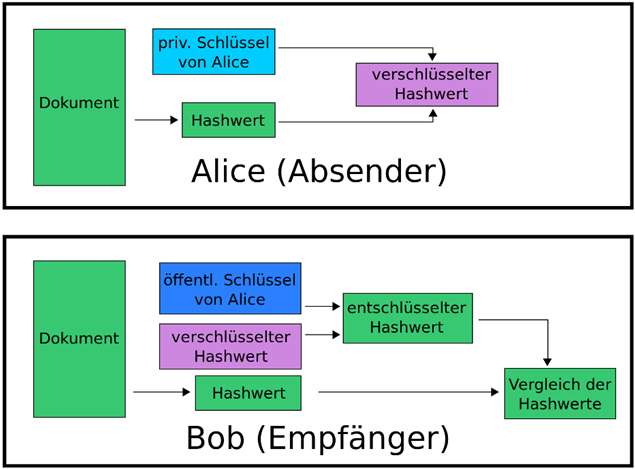
\includegraphics[width=12cm]{images/digisignatur1.png}
    \caption{Signatur im Detail}
    \label{digisig1}
    \end{center}
\end{figure}

\paragraph*{Beispiel}Max Meier erhält von seinem Kunden den Geschäftsvertrag – digital als PDF, wie es heutzutage üblich ist. Vergleichsweise altmodisch geht es aber nachher weiter: Meier druckt das Dokument aus und unterzeichnet es handschriftlich. Den unterschriebenen Vertrag steckt er schliesslich in einen Umschlag und wirft diesen in den nächstgelegenen Briefkasten. Viele Schritte für eine Unterschrift. Was Max Meier nicht weiss: Dokumente lassen sich auch digital unterzeichnen. Jede digitale Signatur basiert auf der sogenannten asymmetrischen Verschlüsselung. Sie wird auch als Public-Key-Verfahren bezeichnet und nutzt einen öffentlichen und einen privaten (geheimen) Schlüssel. Mit dem privaten Schlüssel wird die digitale Signatur erzeugt, während mit dem öffentlichen Schlüssel die Authentizität der Unterschrift überprüft wird.

\paragraph*{Eigenschaft einer Signatur}
\begin{enumerate}[noitemsep,topsep=0pt,leftmargin=*]
    \item \textbf{Fälschungssicherheit:} Nach dem Unterschreiben kann das Dokument nicht mehr (unerkannt) verändert werden.
    \item \textbf{Authentizität:} Die Unterschrift kann zweifelsfrei (überprüfbar) einer bestimmten Person zugeordnet werden.
    \item \textbf{Unleugbarkeit:} Der Unterzeichner kann später nicht abstreiten, das Dokument unterschrieben zu haben.
    \item \textbf{Willenserklärend:} Die Unterschrift kann nur willentlich (bewusst) unter das Dokument gesetzt worden sein.
\end{enumerate}
\begin{figure}[H]
    \begin{center}
    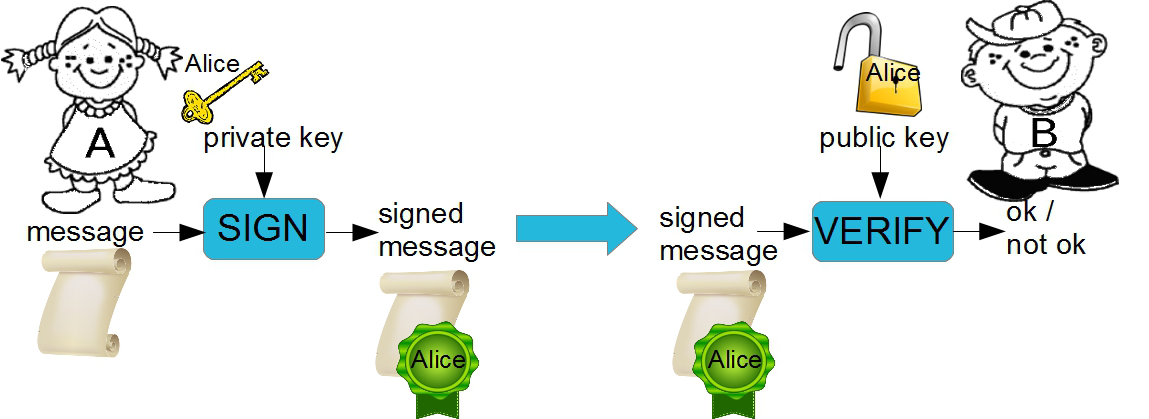
\includegraphics[width=12cm]{images/digisignatur0.png}
    \caption{Alice verschickt eine signierte Nachricht an Bob}
    \label{digisig0}
    \end{center}
\end{figure}


\subsection*{Sie wissen wie hybride Verschlüsselung bzw. hybride Signaturen funktionieren}
\paragraph*{Hybridverschlüsselung}\index{Hybridverschlüsselung}Eine Hybridverschlüsselung ist eine Kombination von symmetrischer und asymmetrischer Verschlüsselung. Dabei werden die Vorteile beider Verschlüsselungsverfahren genutzt. Symmetrische Verschlüsselung ist deutlich schneller, asymmetrische haben den Vorteil eines deutlich einfacheren Schlüsselaustausches. Der Ablauf ist folgendermassen:
\begin{itemize}[noitemsep,topsep=0pt,leftmargin=*]
    \item Sender Alice einen zufälligen symmetrischen Schlüssel, einen Session-Key
    \item Der Session-Key verschlüsselt die Daten/Nachricht symmetrisch
    \item Der Session-Key wird asymmetrisch mit Bob's Public-Key verschlüsselt
    \item Die verschlüsselten Sachen werden an Bob gesendet
    \item Bob entschlüsselt asymmetrisch den Session-Key mit seinem Private-Key
    \item Der Session-Key entschlüsselt nun die Nachricht symmetrisch
\end{itemize}
\begin{figure}[H]
    \begin{center}
    \includegraphics[width=12cm]{images/hybridverschlüsselung.png}
    \caption{Hybridverschlüsselung einer Nachricht}
    \label{hybrid}
    \end{center}
\end{figure}
Man erkennt schnell den Vorteil dieser Methode. Ein symmetrisches Verschlüsselungsverfahren ist sehr effizient auch im Verschlüsseln von grossen Datenmengen

\subsection*{Kontrollfragen SW 03}

\paragraph*{Vergleichen Sie symmetrische und asymmetrische Verschlüsselung bezüglich Anzahl Schlüssel, Schlüssellänge und Geschwindigkeit der Algorithmen}
\begin{itemize}[noitemsep,topsep=0pt,leftmargin=*]
    \item \textbf{Symmetrisch:} 1 Schlüssel, Schlüsselänge eher kürzer, Geschwindigkeit hoch
    \item \textbf{Asymmetrisch:} Mehrere Schlüssel (meistens 2), Schlüssellänge sehr sicher (lang), Geschwindigkeit tief
\end{itemize}

\paragraph*{Warum wird in der Praxis bei der Email-Verschlüsselung ein sog. hybrider Verschlüsselungsalgorithmus angewandt?}\index{Email-Verschlüsselung}\index{Hybrider Verschlüsselungsalgorithmus}Es muss schnell gehen und somit wird auf eine hybride Variante umgestiegen. Dies erhöht die Geschwindigkeit, ohne die Sicherheit zu mindern.


\section{Zertifikate und SSL-TLS}

\subsection*{Sie kennen die verschiedenen Arten von "`Trust"'}
Problematik: Wie ordnet man ein Public Key einer bestimmten Person / Entität zu?
\begin{figure}[H]
    \begin{center}
    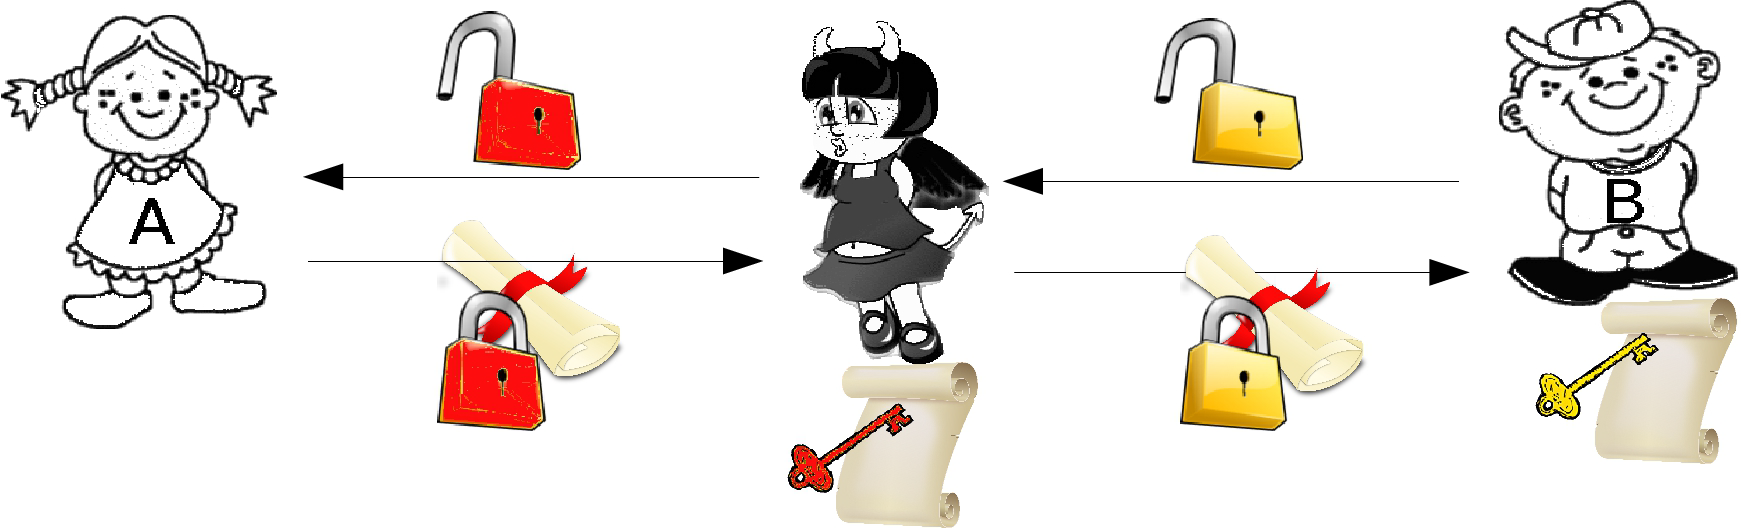
\includegraphics[width=14cm]{images/mitma.png}
    \caption{Eve als man in the middle}
    \label{mitma}
    \end{center}
\end{figure}

\paragraph*{Direct Trust}
Alice vertraut der Authentizität von Bob's Public Key, durch direktes Überprüfen, normalerweise über den Fingerprint des Key's.
\begin{figure}[H]
    \begin{center}
    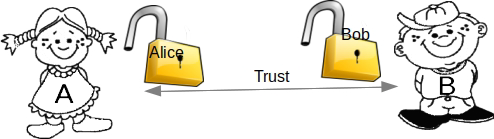
\includegraphics[width=9cm]{images/directtrust.png}
    \caption{Alice vertraut Bob durch direkte Überprüfung}
    \label{directtrust}
    \end{center}
\end{figure}
\begin{itemize}[noitemsep,topsep=0pt,leftmargin=*]
    \item Persönliche Überprüfung
    \item Vorinstalliert in System oder Software (z.B. Public Key von Google-Server in Chrome, Apps, VPN-Clients)
    \item Publiziert auf Webseite oder in Zeitung
\end{itemize}
Benötigt jedoch einen authentischen Kanal zum Etablieren des Trust.

\paragraph*{Web of Trust (WOT)}
Alice vertraut der Authentizität von Daves Public Key, weil dieser von Charlie signiert wurde, dessen Public Key wiederum von Bob signiert wurde, dem sie vertraut.
\begin{figure}[H]
    \begin{center}
    \includegraphics[width=12cm]{images/wot.png}
    \caption{Alice vertraut Dave indirekt durch Vertrauensnetz}
    \label{wot}
    \end{center}
\end{figure}

\paragraph*{Hierarchial Trust (PKI)}Eine \textsl{Public Key Insfrastructure (PKI)} ist ein System, das digitale Zertifikate ausstellen, verteilen und Prüfen kann. Im Gegensatz zum WOT ist eine PKI hierarchisch aufgebaut und bedingt deshalb Root Certification Authorities, welche über alle anderen Zertifizierungstellen steht.
\begin{figure}[H]
    \begin{center}
    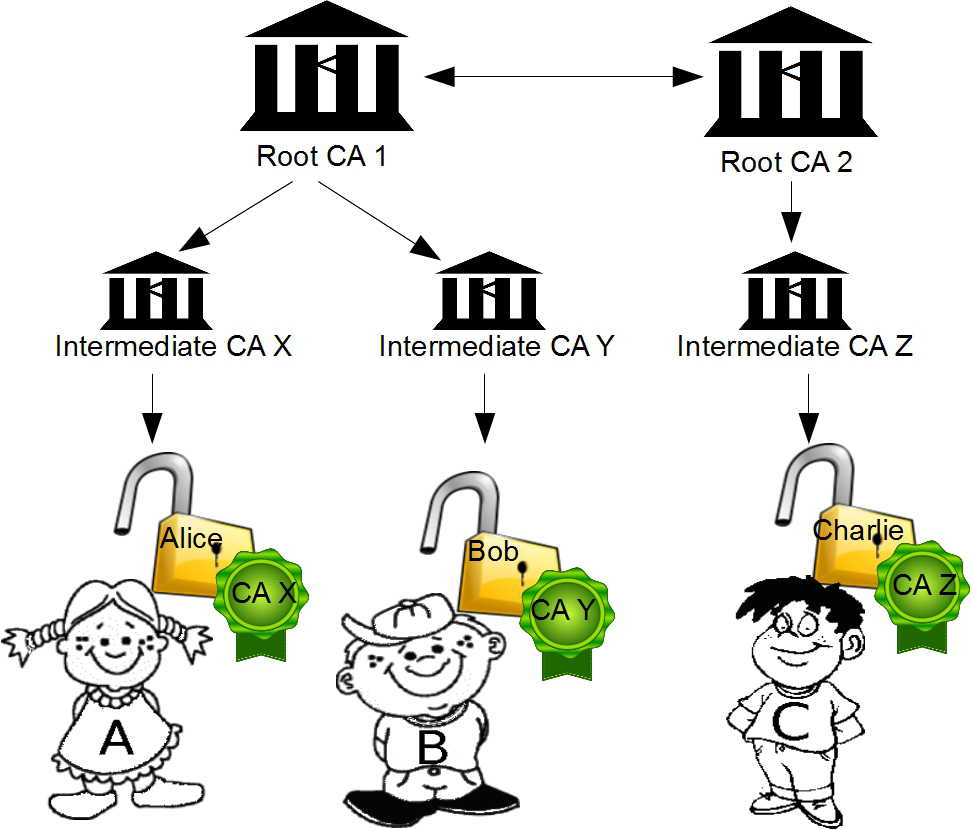
\includegraphics[width=8cm]{images/ht.png}
    \caption{Hierarchical Trust durch Certificate Authorities}
    \label{ht}
    \end{center}
\end{figure}


\subsection*{Sie wissen was eine Public-Key-Infrastruktur, eine Certificate Authority und ein Zertifikat ist, wofür und wie diese verwendet werden und wie Zertifikate ausgestellt und revoziert werden}

\paragraph*{Grundbegriffe PKI}Die Zertifizierungstelle \textsl{Certificate Authority (CA)}\newline
Eine CA ist eine Organistation, welche digital eZertifikate ausstellt. Ein digitales Zertifikat ordnet einen bestimmten öffentlichen Schlüssel einer Person oder Organisation zu. Diese Zuordnung wird von der Zertifizierungstelle beglaubigt, indem sie sie mit ihrer eigenen digitalen Unterschrift versieht.\newline
Ein Zertifikat wird durch eine sog. \textsl{Chain of Trust} beglaubigt. Eine \textsl{intermediate CA} signiert das Zertifikat (Public Key) des Endbenutzers. Das Zertifikat der intermediate CA wird wiederum von einer anderen CA unterschrieben. Das letzte Zertifikat in dieser Kette heisst \textsl{Root Certificate} und enthält den Public Key der \textsl{root CA}. Dieses Zertifikat ist normalerweise \textsl{self signed}, also von der root CA selbst unterschrieben.


\subsection*{Sie wissen was SSL/TLS ist, welche Funktionalität es erreicht und wie das Protokoll konzeptionelle abläuft}SSL-TLS erreicht
\begin{itemize}[noitemsep,topsep=0pt,leftmargin=*]
    \item Authentisierung des Servers gegenüber dem Client
    \item \textsl{Optional}: Authentisierung des Clients gegenüber dem Server (`mutual SSL')
    \item Verschlüsselung und Authentisierung der Daten
\end{itemize}
Das SSL/TLS-Protokoll läuft in \underline{zwei Phasen} ab:
\begin{itemize}[noitemsep,topsep=0pt,leftmargin=*]
    \item \textbf{Handshake}: vereinbart mittels Public-Key-Kryptographie einen Schlüssel
    \item \textbf{Datenaustausch}: verwendet Secret-Key-Kryptographie zum Verschlüsseln und Authentisieren
\end{itemize}
Beispiele für SSL/TLS-ciphers:
\begin{itemize}[noitemsep,topsep=0pt,leftmargin=*]
    \item \verb|TLS_RSA_WITH_3DES_EDE_CBC_SHA|
    \item \verb|TLS_ECDHE_ECDSA_WITH_AES_256_CBC_SHA384|
\end{itemize}

\section*{Kontrollfragen SW 04}
\paragraph*{Was prüfen Sie alles bei einer Authentisierung mittels Zertifikat?}\index{Authentisierung}\index{Zertifikat}
\begin{itemize}[noitemsep,topsep=0pt,leftmargin=*]
    \item Ist das Zertifikat gültig? (Nicht abgelaufen, nicht revoziert)
    \item Ist das Zertifikat und die gesamte Zertifikatskette korrekt signiert?
    \item Traue ich der Root-CA der Zertifikatskette?
    \item Besitzt "`Bob"' den zum Zertifikat gehörenden Private Key?
    \begin{itemize}[noitemsep,topsep=0pt,leftmargin=*]
        \item $VERIFY_{public\,key\,Bob}(response)$
    \end{itemize}
\end{itemize}

\paragraph*{Eine CA hat Ihnen ein Intermediate-CA-Zertifikat ausgestellt, anstelle des bestellten Serverzertifikats. Erklären Sie, wie Sie nun vorgehen, um sich als Google auszugeben. Angenommen Sie können einen Man-in-the-Middle-Angriff machen. Können Sie nun Ihre eigene Webseite anstelle der Google-Seite anzeigen?}
\paragraph*{TODO}


%%%%%%%%%%
\part{Angriffe (SW~05-06)}
\section{Angriffe auf Webanwendungen}

\paragraph*{Bedrohungen auf Anwendungsebene}Webanwendung, Session, Headers, CSRF

\subsection*{Sie wissen was eine Webanwendung ausmacht, wie HTTP funktioniert}
Was unterscheidet eine Webanwendung aus Sicherheitssicht zu anderen Anwendungen?
\begin{itemize}[noitemsep,topsep=0pt,leftmargin=*]
    \item Kommuniziert über HTTP mit einem Server
    \begin{itemize}[noitemsep,topsep=0pt,leftmargin=*]
        \item zustandsloses Protokoll
    \end{itemize}
    \item Läuft in einem Browser
    \begin{itemize}[noitemsep,topsep=0pt,leftmargin=*]
        \item Mehrere Webanwendungen können parallel im gleichen Browser laufen
        \item Die Webanwendung \textsl{erbt} vom Browser implementierte Features
        bzw. muss diese richtig ansprechen
    \end{itemize}
\end{itemize}

\paragraph*{HTTP}Der Browser kommuniziert mit dem Webserver über das \textbf{Hypertext Transfer Protokoll (HTTP)}. HTTP besteht aus \textsl{Requests} und \textsl{Reponses}.

\paragraph*{HTTP-Request-Methoden}Die häufigsten HTTP-Request-Methoden sind \textbf{GET} und \textbf{POST}.
Es existieren aber auch \textbf{PUT, HEAD, DELETE, PATCH, OPTIONS}.

\paragraph*{GET}\verb|https://www.hslu.ch/?p=5 HTTP/1.1|\\
\verb|User-Agent: Mozilla/5.0|
\begin{itemize}[noitemsep,topsep=0pt,leftmargin=*]
    \item Message Body: kein
    \item Ruft Daten vom Server ab
    \item Sollte Serverzustand nicht verändern
\end{itemize}

\paragraph*{POST}\verb|https://www.hslu.ch/ HTTP/1.1|\\
\verb|User-Agent: Mozilla/5.0|
\begin{itemize}[noitemsep,topsep=0pt,leftmargin=*]
    \item Message Body: \verb|id=123&pwd=password|
    \item Darf Serverzustand verändern
    \item Wird nicht gecachet
\end{itemize}

\paragraph*{Häufigste Reponse-Codes}
\begin{itemize}[noitemsep,topsep=0pt,leftmargin=*]
    \item 200 OK
    \item 204 No Content
    \item 301 Moved Permanently
    \item 302 Found (Vorher: "`Moved temporarely"')
    \item 304 Not Modified
    \item 400 Bad Request
    \item 403 Forbidden
    \item 404 Not Found
    \item 500 Internal Server Error
\end{itemize}

\paragraph*{HTTP Zustand} HTTP ist ein zustandsloses Protokoll, d.h. es hat kein `Gedächtnis', bzw. Erinnerung.
\begin{figure}[H]
    \begin{center}
    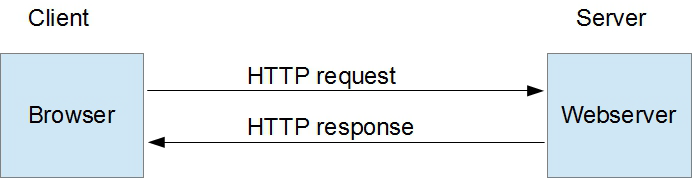
\includegraphics[width=12cm]{images/HTTPZustand0.png}
    \caption{HTTP zustandslos}
    \label{HTTPZustandslos}
    \end{center}
\end{figure}
\noindent
Die einzige Möglichkeit einen Zustand an den Client zu übergeben ist, diesen per weiteren Requests mitzuschicken. Die Zustände werde mit einem Cookie oder einem "`Hidden field"' erfasst.
\begin{figure}[H]
    \begin{center}
    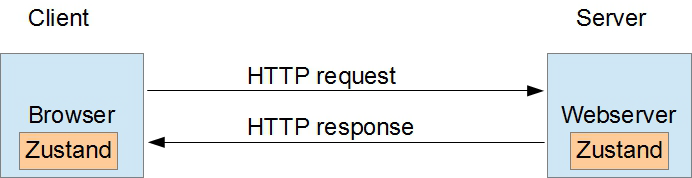
\includegraphics[width=12cm]{images/HTTPZustand1.png}
    \caption{HTTP Zustand per Request (hidden field)}
    \label{HTTPZustand}
    \end{center}
\end{figure}

\paragraph*{Cookies}Cookies sind kurze Textdaten, welche vom Server als Header an den Browser übermittelt werden und von diesem ebenso als Header bei requests wieder mitgesendet werden. Cookies werden vom Browser verwaltet. Die meistgenutzte Möglichkeit ist es, ein Cookie zu setzen. Jedoch dürfen auch Cookies nicht client-seitig angepasst werden können!
\begin{figure}[H]
    \begin{center}
    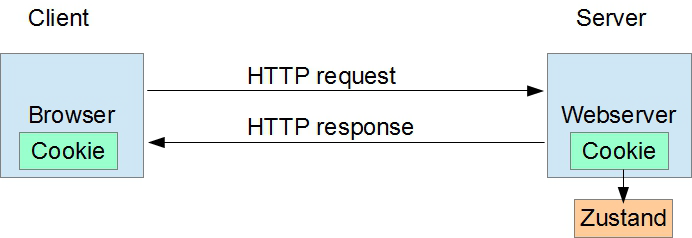
\includegraphics[width=12cm]{images/HTTPCookie.png}
    \caption{Einsatz eines Cookies}
    \label{HTTPCookie}
    \end{center}
\end{figure}

\paragraph*{Cookie Eigenschaften}Die Eigenschaften von Cookies sind:
\begin{itemize}[noitemsep,topsep=0pt,leftmargin=*]
    \item \textbf{Persistent} (mit Ablaufdatum) oder \textbf{Session-Cookie} (ohne Ablaufdatum)
    \item \textbf{Secure} (wird nur über HTTPS übertragen)
    \item \textbf{HTTP Only} (darf nur von HTTP gelesen werden)
    \item \textbf{Same Site} (wird nicht bei Cross-Domain-Aurfrufen mitgesendet, z.B. `embedded' Link, Image)
\end{itemize}


\subsection*{Sie wissen was eine Session ist und welche Eigenschaften einer Session bei welchen Angriffen wichtig sind bzw wie sie gegen gewisse Angriffe Schutz bieten}

\paragraph*{Session} Eine Session ist der Zeitraum, in dem ein Client eine stehende Verbindung mit einem Server hat; vom Login bis zum Logout. Der Server vergibt dem Client eine eindeutige Session-ID. Die Sitzungsdaten (z.B. Warenkorb) werden im Server gespeichert. Bei jedem Request gibt der Client seine Session-ID mit, damit der Server beim Response die zugehörigen Daten dieser ID übermitteln kann. Es gibt auch Sessions ohne stehende Verbindung (ohne Login). Dies wird zu Statistikzwecken verwendet, z.B. um die Bewegung des Besuchers auf der Website zu verfolgen. Oder aber auch um einen Warenkorb ohne Login verwenden zu können.

\paragraph*{Schwaches Session-Management}Was ist das?
\begin{itemize}[noitemsep,topsep=0pt,leftmargin=*]
    \item der Sessionwert ist vorhersagbar
    \item der Sessionwert kann vom Client gesetzt werden
    \item die Cookie-Attribute `Secure', `HttpOnly' oder `Same Site' sind nicht gesetzt
    \item Cookie-Domain oder -Pfad sind nicht so eingeschränkt wie möglich
    \item die Session wird bei einem Logout nicht invalidiert
    \item die Session hat kein server-seitiges Timeout (Inaktivitäts- und absolutes Timeout)
\end{itemize}

\paragraph*{Schwaches Session-Management}Was kann man dagegen tun?
\begin{itemize}[noitemsep,topsep=0pt,leftmargin=*]
    \item lange und kryptographisch zufällige Sessionwerte wählen
    \item nur vom Server gewählte Sessionwerte akzeptieren
    \item Cookies als `Secure',`HttpOnly' oder `Same Site' mit so eingeschränkter Domain und Pfad wie möglich setzten
    \item Session \textbf{server-seitig} bei einem Logout oder Timeout invalidieren
\end{itemize}

\paragraph*{Same Origin Policy}Mehrere Webanwendungen können im gleichen Browser parallel laufen. Die Same-Origin-Policy verhindert, dass eine parallel laufende Webanwendungen uneingeschränkt
\begin{itemize}[noitemsep,topsep=0pt,leftmargin=*]
    \item auf die Daten einer anderen Anwendung zugreifen
    \item die Cookies einer anderen Anwendung lesen oder mitschicken
    \item Requests auf die andere Anwendung absetzen
\end{itemize} kann.\\
Same Origin Policies im Browser gibt es z.B. für Cookies, DOM access (Zugang zu document.cookie), HTML5Storage, XMLHttpRequests.

\paragraph*{Same Origin Policy: Cookies} Cookies haben eine \textbf{domain} und \textbf{path}.
\begin{itemize}[noitemsep,topsep=0pt,leftmargin=*]
    \item \textbf{Setzen des Cookies:} Nur Domain-Suffix des URL-Hostname dürfen gesetzt werden. (Aber keine Top-Level Domains!)\\
    Path kann beliebig gesetzt werden.
    \item \textbf{Senden des Cookies:} Cookies werden dnur dann mitgeschickt, wenn die Cookie-Domain ein Domain-Suffix der URL-Domain und der Cookie-Path ein Prefix des URL-Path ist.
\end{itemize}

\paragraph*{Session Fixation}Was ist das?\\
Der Sessionwert wird nach einem Login oder Loginschritt nicht geändert. Ein  angreifer mit Zugang zu einer unauthentisierten Session kann warten bis ein Benutzer sich einloggt und ist damit selbst eingeloggt.

\paragraph*{Session Fixation}Was kann man dagegen tun?\\
Sessionwert nach jedem Authentisierungsschritt ändern.

\subsection*{Sie kennen sicherheitsrelevante Header}

\paragraph*{Sicherheitsrelevante Response-Header}
\begin{enumerate}[noitemsep,topsep=0pt,leftmargin=*]
    \item \textbf{HSTS:} \verb|Strict-Transport-Security: max-age=31536000; includeSubDomains|\\
    Seite wird nur via HTTPS aufgerufen. \verb|max-age| muss hoch gesetzt werden!
    \item \textbf{Frame-Options:} \verb|X-Frame-Options: deny|\\
    Verbietet das Einbinden der Seite in einem Frame oder erlaub es nur für bestimmte Domains
    \item \textbf{XSS-Protection:} \verb|X-XSS-Protection: 1; mode=block|\\
    Filtert und säubert oder blockeirt die Anzeige der Seide, wenn ein XSS-Angriff endeckt wird
    \item \textbf{Content-Type-Options:} \verb|X-Content-Type-Options: nosniff|\\
    Verhindert, dass der Content als einen anderen MIME-Type interpretiert wird als angegeben
    \item \textbf{CSP:} \verb|Content-Security-Policy: script-src \textquotesingle self\textquotesingle|\\
    Definiert, welche Resourcen (z.B. Bilder, Scripts, Fonts, etc.) von wo eingebunden werden können
    \item \textbf{CORS} \verb|Access-Control-Allow-Origin: http://foo.example|\\
    Cross-Origin Resource Sharing (CORS) ist ein Mechanismus, der Webbrowsern oder auch anderen Webclients Cross-Origin-Requests ermöglicht. Zugriffe dieser Art sind normalerweise durch die Same-Origin-Policy (SOP) untersagt. CORS ist ein Kompromiss zugunsten grösserer Flexibilität im Internet unter Berücksichtigung möglichst hoher Sicherheitsmassnahmen.
    \item \textbf{Caching-Options} {\color{red}TODO: hat jemand Infos?}
    \item \textbf{HPKP ({\color{red}deprecated!}):}
    \verb|Public-Key-Pins:|\\
    \verb|pin-sha256="d6qzRu9zOECb90Uez27xWltNsj0e1Md7GkYYkVoZWmM=";|\\
    \verb|pin-sha256="Ë9CZ9INDbd+2eRQozYqqbQ2yXLVKB9+xcprMF+44U1g=";|\\
    \verb|report-uri=http://example.com/pkp-report;|\\
    \verb|max-age=10000; includeSubDomains|\\
    HTTP Public Key Pinning: Nur das Serverzertifikat mit dem korrekten Fingerprint wird akzeptiert. Wurde wieder abgekündigt und die meisten Browser unterstützen es nicht mehr.
\end{enumerate}

\subsection*{Sie verstehen wie ein Cross-Site-Request-Forgery-Angriff abläuft und wie man sich dagegen schützen kann}

\paragraph*{CSRF - Cross-Site Request Forgery}Was ist das?\\
Der Angreifer bringt einen Benutzer dazu, einen Request aus seinem Browser abzusetzen und  dadurch eine Aktion auf dem Server auszulösen. Ist der Benutzer zu dem Zeitpunkt eingeloggt, wird das Cookie automatisch mitgeschickt.
\begin{figure}[H]
    \begin{center}
    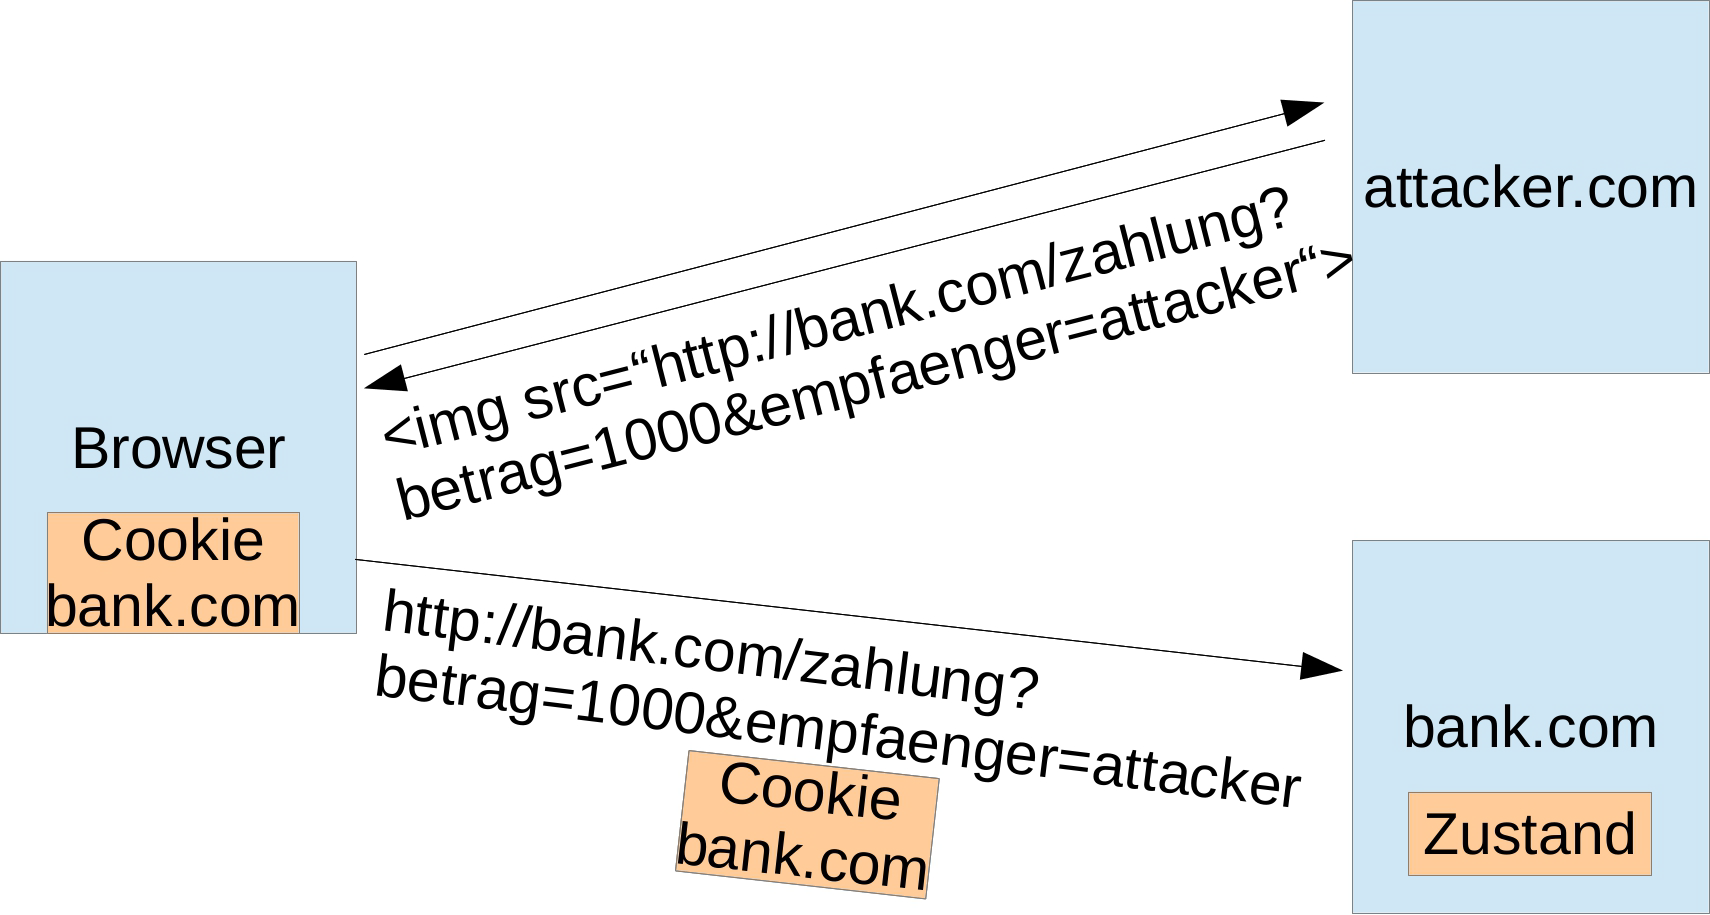
\includegraphics[width=10cm]{images/CSRF.png}
    \caption{Cross-Site Request Forgery}
    \label{CSRF}
    \end{center}
\end{figure}
\paragraph*{CSRF - Cross-Site Request Forgery}Was kann man dagegen tun?
\begin{itemize}[noitemsep,topsep=0pt,leftmargin=*]
    \item \textbf{CSRF-Token:} ein Secret als Teil des Form Field oder Header mitgeben (Secret darf nicht vorhersagbar sein)
    \item \textbf{Zusätzlich:} Same-Site-Attribut setzten
\end{itemize}


\section{Angriffe auf Protokollebene}
\subsection*{Sie kennen die Grundbegriffe der Anwendungssicherheit}
\paragraph*{Bedrohungen auf Protokollebene}Begriffe: Social Engineering, Angriffe auf ARP, TCP/IP, DNS, SSL, HTTP

\subsection*{Kurzübersicht}
\index{Bedrohungen auf OSI-Layern}
\begin{itemize}[noitemsep,topsep=0pt,leftmargin=*]
    \item \textbf{Bedrohungen auf Link-Layer:} Spoofing\index{Link-Layer}\index{Spoofing}
    \item \textbf{Bedrohungen auf Transport-Layer:} Denial of Service (DoS)\index{Transport-Layer}\index{DoS}
    \item \textbf{Bedrohungen auf SSL / TLS:} Preisgabe Sensitiver Daten\index{SSL/TLS}\index{Sensitive Daten}
    \item \textbf{Bedrohungen auf Anwendungslayer:} Cross Site Scripting (XSS), Code Injection\index{Anwendungslayer}\index{Cross Site Scripting (XSS)}\index{Code-Injection}\index{XSS! siehe {Cross Site Scripting (XSS)}}
    \item \textbf{Bedrohungen auf Layer 8 (Mensch):} Social Engineering\index{Layer 8}\index{Social Engineering}
\end{itemize}

\index{Fehler vs. Bugs}
\paragraph*{Flaws vs. Bugs} Bei Softwaredefekten wird unterschieden zwischen Flaws und Bugs
\begin{itemize}[noitemsep,topsep=0pt,leftmargin=*]
    \item \textbf{Flaw:} Ein Flaw ist ein Defekt im Design der Software\index{Flaw}
    \item \textbf{Bug:} Ein Bug ist ein Defekt in der Implementation\index{Bug}
\end{itemize}

\paragraph*{Grundbegriffe: Bedrohung}
\index{Threat vs. Threat Agent}\index{Threat}
\begin{itemize}[noitemsep,topsep=0pt,leftmargin=*]
    \item \textbf{Threat:} Möglicher Grund für einen ungewollten Vorfall, der das System oder die Organisation schädigen kann.
    \item \textbf{Threat Agent:} Individuum oder Gruppe welche eine Bedrohung darstellt.
\end{itemize}

\index{Aktive vs. Passive Angriffe}
\subsubsection*{Aktive vs. passive Angriffe}
Bei einem \textbf{passiven Angriff} hält sich der Angreifer an das protokoll. Er verändert z.B. die ausgetauschten Nachrichten nicht hört aber die Kommunikation ab.
Bei einem \textbf{aktiven Angriff} hält sich der Angreiffer nicht an das Protokoll. Er verändert z.B. Nachrichten.

\subsection*{Sie kennen Beispiele von Angriffen auf verschiedenen Ebenen des Protokollstacks und wissen was diese bewirken}

\index{OSI-Modell}
\subsubsection*{OSI-Layers}
Die 7 Tierschichten des OSI-Models, wobei die 8te sich auf den Mensch bezieht.

\begin{figure}[H]
    \begin{center}
    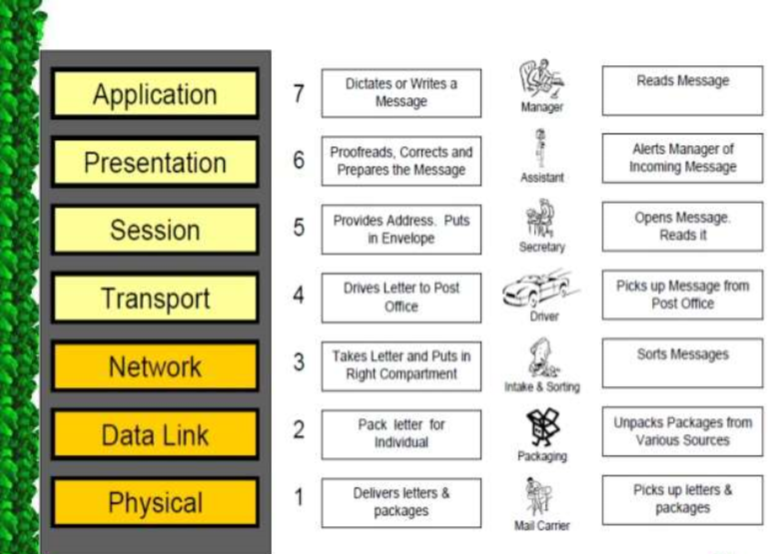
\includegraphics[width=8cm]{images/OSI-Layers.png}
    \caption{OSI-Layers}
    \label{OSI-Layers}
    \end{center}
\end{figure}

\subsubsection*{OSI vs Internet Reference Model}
Die 7 Tierschicht des OSI-Models, wobei die 8te sich auf den Mensch bezieht.

\begin{figure}[H]
    \begin{center}
    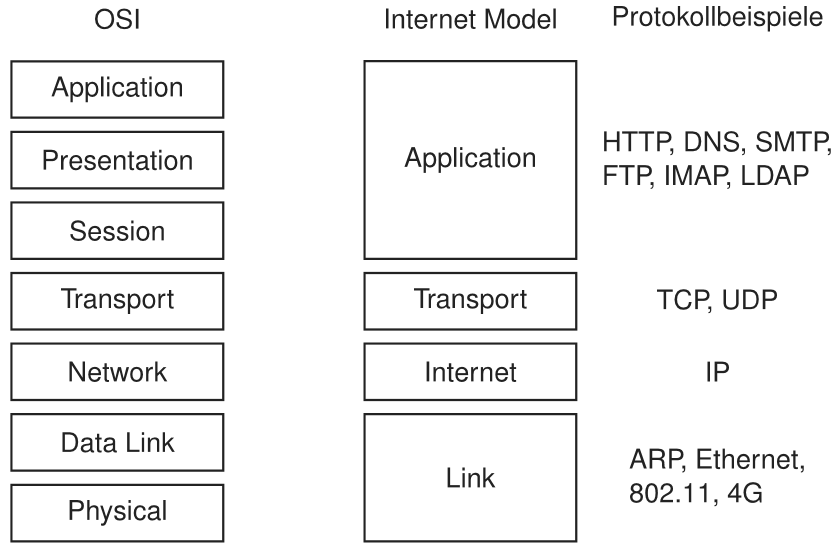
\includegraphics[width=8cm]{images/OSIvsIRM.png}
    \caption{OSI vs. Internet Reference Model}
    \label{OSIvsIRM}
    \end{center}
\end{figure}


\subsubsection*{Encapsulation (Datenkapselung)}
\begin{figure}[H]
    \begin{center}
    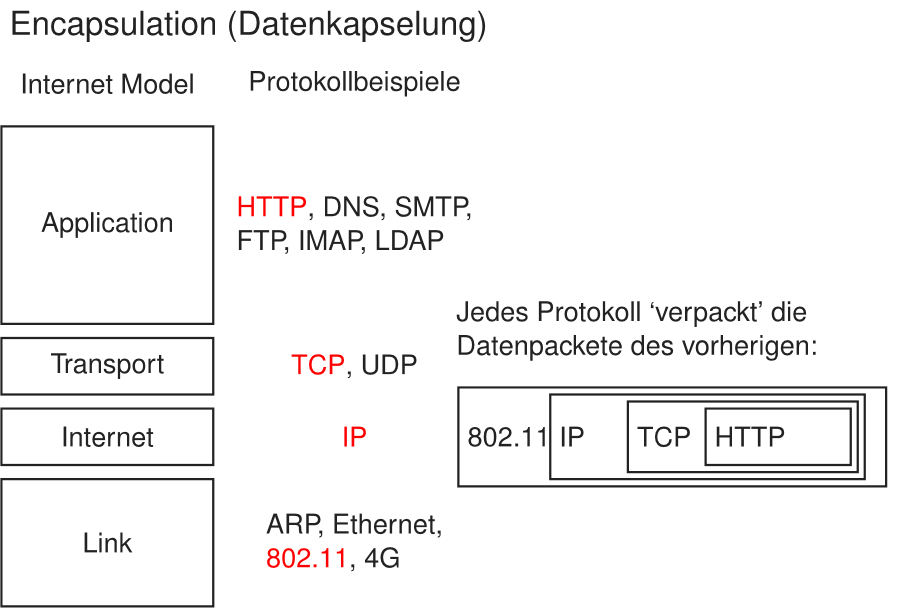
\includegraphics[width=8cm]{images/TCP-Encapsulation.png}
    \caption{TCP-Encapsulation}
    \label{TCP-Encapsulation}
    \end{center}
\end{figure}

\index{ARP-Spoofing}
\subsubsection*{Beispiel: ARP-Spoofing auf dem Link-Layer}
\begin{figure}[H]
    \begin{center}
    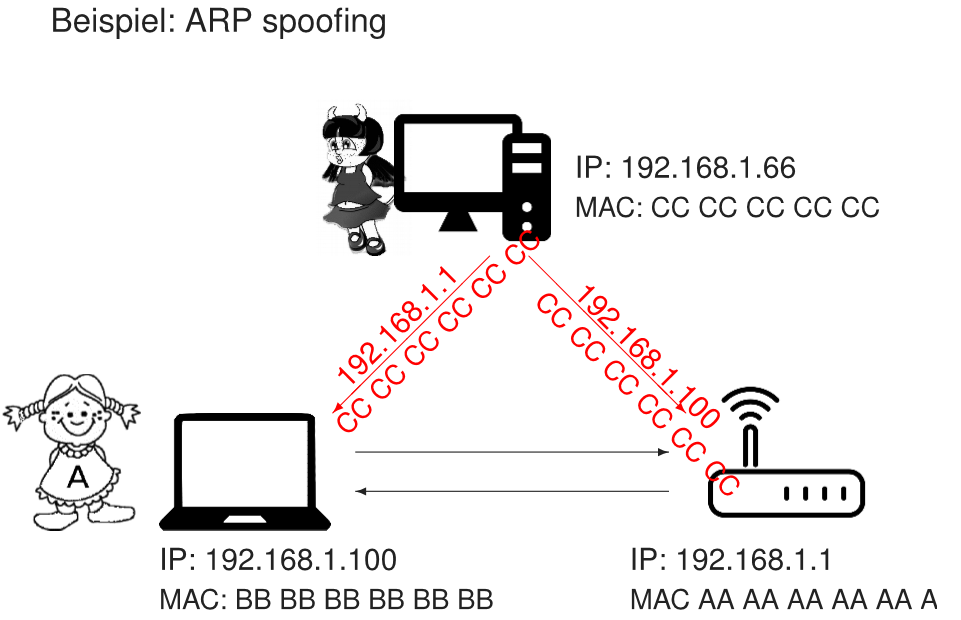
\includegraphics[width=8cm]{images/Beispiel_ARP_Spoofing.png}
    \caption{ARP Spoofing}
    \label{ARP Spoofing}
    \end{center}
\end{figure}

\paragraph*{Spoofing: Was ist das?}
Eine person oder ein Programm gibt sich als jemand anderen oder etwas anderes aus.\\
\textbf{Beispiele:}
\begin{itemize}[noitemsep,topsep=0pt,leftmargin=*]
    \item \textbf{Telefonnummern-Spoofing (Call Centers etc.)}
    \item \textbf{Email-Adressen-Spoofing}
    \item \textbf{IP Spoofing}
    \item \textbf{DNS Spoofing}
    \item \textbf{ARP Spoofing}
    \item \textbf{Content Spoofing}
\end{itemize}
\vspace{0.5cm}
\noindent
"`\textsl{ARP-Spoofing (vom engl. to spoof – dt. täuschen, reinlegen) oder auch ARP Request Poisoning (zu dt. etwa Anfrageverfälschung) bezeichnet das Senden von gefälschten ARP-Paketen. Es wird benutzt, um die ARP-Tabellen in einem Netzwerk so zu verändern, dass anschließend der Datenverkehr zwischen zwei (oder mehr) Systemen in einem Computernetz abgehört oder manipuliert werden kann. Es ist eine Möglichkeit, einen Man-in-the-Middle-Angriff im lokalen Netz durchzuführen.}"' - Wikipedia

\paragraph*{Spoofing: Was kann man dagegen tun?}
\paragraph*{Je nach Situation unterschiedlich, zB.:}
\begin{itemize}[noitemsep,topsep=0pt,leftmargin=*]
    \item {Authentisieren}
    \item {Angaben überprüfen}
\end{itemize}

%
\index{3-Way Handshake} \index{TCP Verbindungsaufbau}
\subsubsection*{Repetition: TCP Verbindungsaufbau (vereinfacht)}
\begin{figure}[H]
    \begin{center}
    \includegraphics[width=8cm]{images/Repetition_3_way_handshake.png}
    \caption{3-Way Handshake}
    \label{3-Way Handshake}
    \end{center}
\end{figure}

\index{DoS}
\paragraph*{Bedrohungen auf Transport-Layer:} Denial of Service (DoS)
\paragraph*{Denial of Service}Syn-Nachrichten werden mit gespoofter IP gesendet. Syn-Acknowledgements Nachrichten gehen nirgendwo hin.
Server wird überflutet mit Abfragen und kann nicht schneller abarbeiten als Sie reinkommen.
Als Resultat kann somit von den meisten Benutzern die Seite nicht angezeigt werden.
\begin{figure}[H]
    \begin{center}
    \includegraphics[width=8cm]{images/Syn-flood.png}
    \caption{SYN Flood}
    \label{Syn Flood}
    \end{center}
\end{figure}

\index{DRDoS}
\paragraph*{Beispiel: Distributed Reflection Denial of Service}
\noindent
"`\textsl{Hierbei adressiert der Angreifer seine Datenpakete nicht direkt an das Opfer, sondern an regulär arbeitende Internetdienste, trägt jedoch als Absenderadresse die des Opfers ein (IP-Spoofing). Die Antworten auf diese Anfragen stellen dann für das Opfer den eigentlichen DoS-Angriff dar. Durch diese Vorgehensweise ist der Ursprung des Angriffs für den Angegriffenen nicht mehr direkt ermittelbar.}"' - Wikipedia

\begin{figure}[H]
    \begin{center}
    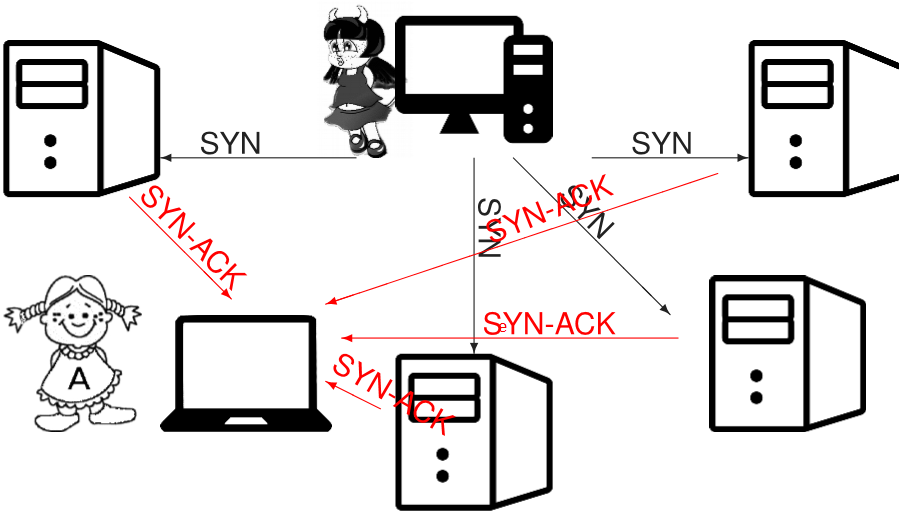
\includegraphics[width=8cm]{images/DRDoS.png}
    \caption{DRDoS}
    \label{DRDoS}
    \end{center}
\end{figure}

\paragraph*{Denial of Service: Was kann man dagegen tun?} Jedes system bricht irgendwann zusammen! Es geht darum sicherzustellen, dass dabei keine bleibenden Schäden am
Kernsystem entstehen und das system nach einem Angriff schnell wieder funktionsfähig zu machen.

\subsubsection*{Schutzbeispiele:}
\begin{itemize}[noitemsep,topsep=0pt,leftmargin=*]
    \item \textbf{Beschränkung der Anzahl (Web-) Requests pro Zeiteinheit / IP }
    \item \textbf{Sicherstellen, dass der "`Flaschenhals"' weit vorne auftritt (z.B. Firewall) um Kernsysteme zu schützen}
    \item \textbf{Sicherstellen, dass das System sich nicht selbst überlastet durch freigeben nicht mehr verwendeter Ressourcen, vermeiden von undendlichen Loops etc.}
    \item \textbf{Disaster Recovery Plan}
\end{itemize}

\subsubsection*{SSL/TLS im internet Modell}\index{SSL/TLS}
\begin{figure}[H]
    \begin{center}
    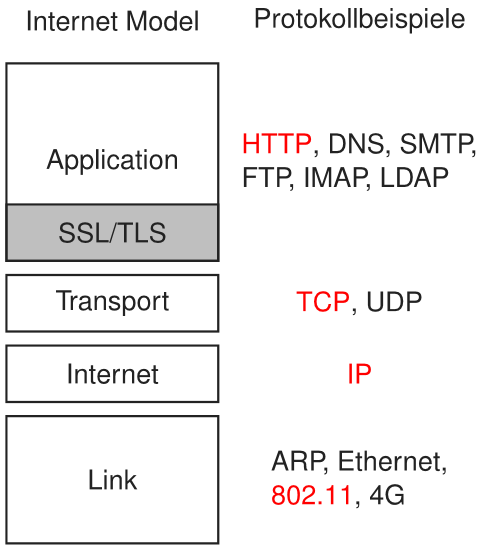
\includegraphics[width=8cm]{images/SSL-TLS.png}
    \caption{SSl/TLS}
    \label{SSL/TLS}
    \end{center}
\end{figure}

\subsubsection*{Bedrohung auf SSL / TLS (Preigabe Sensitiver Daten)}

\index{Sensitive Daten}
\paragraph*{Preisgaber Sensitiver Daten: Was ist das?} Angreifer stehlen Schlüssel, Passwörter, Geschäftsgeheimnsisse,
Personendaten oder andere sensitive Daten vom Server, bei der Übertragung oder vom Client

\paragraph*{Preisgabe sensitiver Daten: Was kann man dagegen tun?}
\begin{itemize}[noitemsep,topsep=0pt,leftmargin=*]
    \item Keine Daten speichern oder übertragen, welche nicht benötigt werden.
    \item Daten nach ihrer Sensivität klassifizieren und entsprechend behandeln
    \item Sensitive Daten nur gespeichert auf dem Server ablegen
    \item Passwörter mit Salt und Pepper und einer starken Passwort-Hashfunktion gehasht ablegen.
    \item Daten verschlüsselt übertragen (FTP \textgreater SFTP,HTTP \textgreater HTTPS, etc). Zertifikat überprüfen!
    \item Sicherstellen, dass sichere Ciphers verwendet werden
    \item Keine sensitiven Daten auf der Clientseite cachen.
\end{itemize}

\subsubsection*{Bedrohungen auf Anwendungslayer: Cross Site Scripting (XSS) und Code Injection}
\index{Cross Site Scripting (XSS)}\index{XSS! siehe {Cross Site Scripting (XSS)}}
\paragraph*{XSS: Was ist das?}Ein Angreifer bringt den legitimen Server dazu ein Script an den Browser zu senden. Dieses wird im Kontext des legitimen Servers ausgeführt. Es wird zwischen \textbf{stored} und \textbf{reflected} XSS unterschieden
\begin{figure}[H]
    \begin{center}
    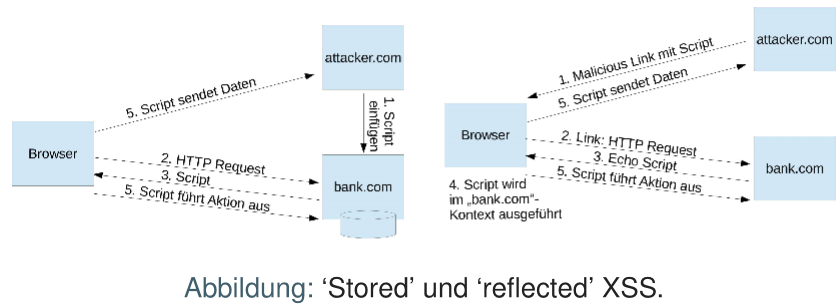
\includegraphics[width=15cm]{images/XSS.png}
    \caption{XSS}
    \label{XSS}
    \end{center}
\end{figure}

\paragraph*{XSS: was kann man dagegen tun?}
\begin{itemize}[noitemsep,topsep=0pt,leftmargin=*]
    \item \textbf {Escaping} aller unsicheren Daten (z.B. vom Benutzer eingegebene) bevor sie angezeigt werden.\\ Bsp. Ersetzen von \textbf{\& \textless \textgreater \textquotedblleft \textquoteright} durch \textbf{\&amp; \&lt; \&gt; \&quot; \&\#x27; \&\#x2F;}
\end{itemize}
\paragraph*{}Zusätzlich sollen folgende Massnahmen getroffen werden:
\begin{itemize}[noitemsep,topsep=0pt,leftmargin=*]
    \item Cookie als HttpOnly-Cookie setzen
    \item Header-Felder setzen\\ Bsp. Content-Security-Policy: default-src: 'self'; script-src: 'self' static.domain.tld \\ Bsp. X-XSS-Protection: 1; mode=block
\end{itemize}

\index{Code Injection}
\paragraph*{Code Injection: Was ist das?} Vermischung von 'Code' und 'Daten'
\begin{figure}[H]
    \begin{center}
    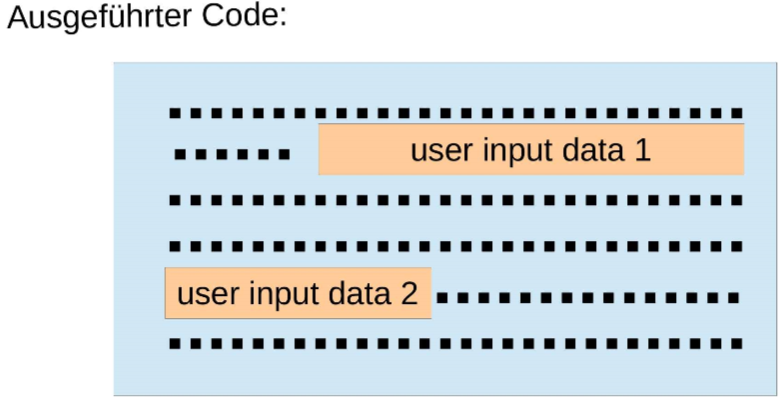
\includegraphics[width=8cm]{images/Code-Injection.png}
    \caption{Code Injection}
    \label{Code Injection}
    \end{center}
\end{figure}

\begin{figure}[H]
    \begin{center}
    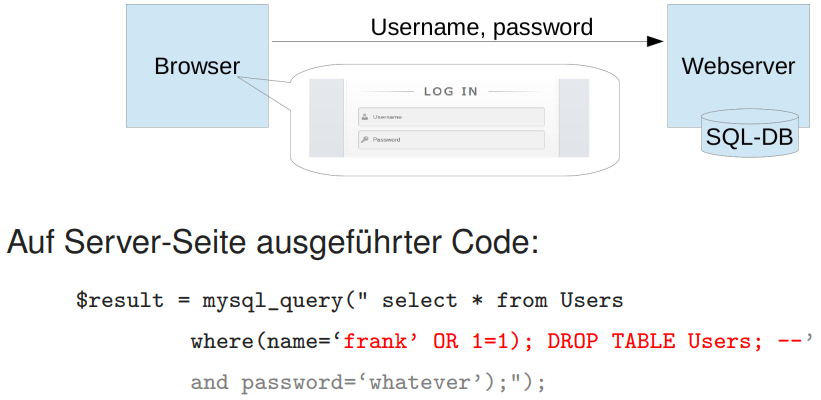
\includegraphics[width=12cm]{images/Bsp-Code-Injection.png}
    \caption{Beispiel Code Injection}
    \label{Code Injection example}
    \end{center}
\end{figure}

\paragraph*{Code Injection: Was kann man dagegen tun?}
\begin{itemize}[noitemsep,topsep=0pt,leftmargin=*]
    \item `Prepared statements' verwenden \\ Beispiel:\\
    \verb|$statement = $db->prepare('SELECT * FROM Users WHERE(name=? password=?);';|\\
    \verb|$stmt->bind_param('ss', $user, $pass);|
    \item Whitelisting der Inputs
    \item Sanitizing der Inputs \\ Bsp. Löschen von Zeichen wie \verb|';-| oder Ersetzen durch `sichere' Zeichen wie \verb|\'\;\-|
    \item Rechte des technischen Benutzers auf der DB einschränken
    \item Verwenden eines sicheren APIs
\end{itemize}

\index{Layer 8}\index{Layer 8}
\subsubsection*{Layer 8}
\begin{figure}[H]
    \begin{center}
    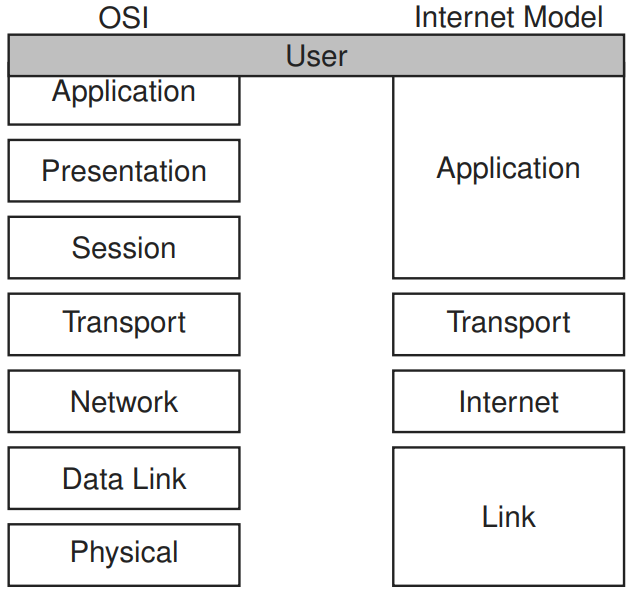
\includegraphics[width=8cm]{images/Layer8.png}
    \caption{Layer 8, der User}
    \label{Layer 8}
    \end{center}
\end{figure}

\index{Social Engineering}
\paragraph*{Social Engineering: Was ist das?}Zwischenmenschliche Beeinflussungen mit dem Ziel, bei
Personen bestimmte Verhaltensweisen hervorzurufen, sie zum
Beispiel zur Preisgabe von vertraulichen Informationen, zum
Kauf eines Produktes oder zur Freigabe von Finanzmitteln zu
bewegen.

\paragraph*{Social Engineering: Was kann man dagegen tun?}
\begin{itemize}[noitemsep,topsep=0pt,leftmargin=*]
    \item Benutzer schulen ('awareness')
    \item Für den Benutzer verständliche Abläufe Sicherstellen
    \item Benutzer nicht zum Umgehen von Sicherheitsmassnahmen verleiten
    \item Fraud Detection-Massnahmen
    \item Technische Massnahmen welche den Angriff verhindern, z.B. Vereinzelungsanlage, nicht vorlesbare Codes etc.
\end{itemize}



\paragraph*{TODO}


%%%%%%%%%%
\part{Management (SW~07-09)}
\section{Standards \& Frameworks, ISMS}

\subsection*{Sie wissen, was ein ISMS ist und wie man damit umgeht}
\paragraph*{ISMS}Ein \textsl{Information Security Management System (ISMS)} (auf Deutsch: Managementsystem für die Informationssicherheit) definiert Regeln, Methoden und Abläufe, um die IT-Sicherheit in einem Unternehmen zu gewährleisten, zu steuern, zu kontrollieren und zu optimieren.
\paragraph*{Zweck}
\begin{itemize}[noitemsep,topsep=0pt,leftmargin=*]
    \item Die (durch die IT verursachte) Risiken sollen identifizierbar und beherrschbar werden.
    \item Sicherheit erhalten, dass teure Informationen und Daten der Unternehmung angemessen geschützt sind.
    \item Rechtliche (Datenschutz- oder Berufsgesetz bei Ärzten / Anwälte) und auch Marktanforderung erfüllen (wenn morgen in den Medien publik wird, dass bei der UBS Bank «gehakt» und Millionen gestohlen wurde, dann würden die Kunden nicht länger ihr Vermögen bei der UBS deponieren.
\end{itemize}
\paragraph*{Vorgehen}
\begin{itemize}[noitemsep,topsep=0pt,leftmargin=*]
    \item Man sollte einen Prozess unterhalten, mit dem die Risiken der Informationssicherheit identifiziert und bewertet werden können. Dazu sollen Kontrollen bestimmt, eingeführt und stetig verbessert werden können.
    \item Davor muss zuerst der Schutzbedarf von Vermögenswerten bestimmt und Schutzmassnahmen eingeführt werden.
\end{itemize}


\subsection*{Sie kennen die wichtigsten Standards der Informationssicherheit}
\paragraph*{Standards}
\begin{itemize}[noitemsep,topsep=0pt,leftmargin=*]
    \item ISO 27000: ISMS – Overview and vocabulary (Überblick / Index)
    \item ISO 27001: ISMS – Requirements (Anforderungskatalog)
    \item ISO 27002: Code of practice for information security controls (Analog: Kochbuch; darin steht drin, welche Massnahmen ich tätigen muss)
    \item ISO 27003: implementation guidance (wie ich die Anforderung umsetze)
    \item ISO 27004: Information security management – Measurement (Ziele müssen messbar sein, z.B. Jahresziele beim Mitarbeiter Gespräch; Ende Periode kann überprüft werden, ob die Ziele erreicht wurden
    \item ISO 27005: Information security risk management (Risiko Bewältigung)
\end{itemize}

\subsection*{Sie finden sich in den Standards ISO 27001 und 27002 zurecht}
\paragraph*{TODO}

\subsection*{Sie verstehen die Grundzüge der BSI-Standards (BSI=Bundesamt für Sicherheit in der Informationstechnik, Deutschland)}
\paragraph*{TODO}

\subsection*{Sie kennen die Struktur und Grundziele des NIST CyberSecurityFrameworks}
\paragraph*{TODO}


\section{Risiko-Management und IT-Grundschutz}
\subsection*{Das Risikoanalyse-Verfahren verstehen}
\paragraph*{TODO}

\subsection*{Die Unterschiede zum Grundschutzverfahren kennen}
\paragraph*{TODO}

\subsection*{Eine einfache Risikoanalyse durchführen können}
\paragraph*{TODO}

\subsection*{Sie verstehen die Idee, die Ziele und die Konzepte des IT-Grundschutz-Vorgehens}
\paragraph*{TODO}

\subsection*{Sie kennen den Aufbau der IT-Grundschutz-Kataloge und deren Anwendungsweise}
\paragraph*{TODO}

\subsection*{Sie können die Teilschritte zum Aufbau eines Sicherheitskonzeptes nach IT-Grundschutz durchführen, kombinierte Risikoanalyse}
\paragraph*{TODO}


\section{Awareness}
\subsection*{Sie verstehen die Wichtigkeit der \flqq Awareness \frqq}
\paragraph*{TODO}

\subsection*{Sie kennen verschiedene Prozesse und Vorgehensweisen für die Initiierung, Durchführung und Erfolgsprüfung einer Awareness-Kampagne und können diese anwenden}
\paragraph*{TODO}

\subsection*{Sie kennen die relevanten Erfolgsfaktorender Mitarbeiter-Sensibilisierung und -Schulung und können diese in einer Kampagne umsetzen}
\paragraph*{TODO}


%%%%%%%%%%
\part{Access Control (SW~10)}
\section{Access Control}
\subsection*{Sie kennen verschiedene Arten der Authentisierung, wissen wie diese technisch ablaufen und was deren Vor- und Nachteile sind}
\paragraph*{TODO}

\subsection*{Sie wissen wie verschiedene Authentisierungstoken technisch funktionieren, was deren Vor- und Nachteile sind und wie sie beim Login oder bei der Transaktionsbestätigung im e-Banking eingesetzt werden}
\paragraph*{TODO}

\subsection*{Sie wissen was Authentisierung, Autorisierung ist, warum diese wichtig sind und wie Angriffe darauf ablaufen}
\paragraph*{TODO}


%%%%%%%%%%
\part{Multi-Party-Computation (SW~11)}
\section{Cryptographic Protocols}
\subsection*{Sie kennen einfache Beispiele von verteilten sicheren Berechnungen und verstehen wie die entsprechenden Protokolle ablaufen}
\paragraph*{TODO}

\section{Secret Sharing}
\subsection*{Sie kennen Arten von Sicherheit von verteilten sicheren Berechnungen und wie diese angegriffen werden können}
\paragraph*{TODO}

\subsection*{Sie wissen welche Eigenschaften elektronisches Geld ausmachen und kennen die technischen Grundlagen von Bitcoin}
\paragraph*{TODO}

\section{Zero Knowledge Proof}
\subsection*{Sie wissen was Zero-Knowledge-Proofs sind und wie diese ablaufen}
\paragraph*{TODO}


%%%%%%%%%%
\part{Quantum (SW~12)}
\section{Quantum Computing and Quantum Cryptography}
\subsection*{Sie wissen was ein Quantencomputer ist und was ihn von einem "`klassischen"' Computer unterscheidet}
\paragraph*{TODO}

\subsection*{Sie verstehen welchen Einfluss die Existenz eines Quantencomputers auf die Kryptographie hat}
\paragraph*{TODO}

\subsection*{Sie verstehen wie Quantenschlüsselaustausch funktionert}
\paragraph*{TODO}


%%%%%%%%%%
\part{WAF, Federations (SW~13)}
\section{Firewalls}
\subsection*{Sie wissen was die Aufgaben einer Firewall sind}
\paragraph*{Aufgaben einer Firewall}Filtern der ein- (WAF) und ausgehenden (HTTP Proxy) Kommunikation nach
\begin{itemize}[noitemsep,topsep=0pt,leftmargin=*]
    \item \textbf{Service control:} Z.B. Protokoll, Portnummer, IP-Adresse
    \item \textbf{Direction control:} Wer hat die Verbindung aufgebaut bzw. den Service initiiert?
    \item \textbf{User control:} Welcher Benutzer versucht einen bestimmten Service auszuführen?
    \item \textbf{Behaviour control:} Wie wird ein Service verwendet? Z.B. Spam-Filter
\end{itemize}

\subsection*{Sie verstehen die Funktionsweise einer WAF und wie sie eine Webanwendung vor Angriffen schützen kann}
\paragraph*{WAF}Funktionalitäten einer Web Application Firewall
\begin{itemize}[noitemsep,topsep=0pt,leftmargin=*]
    \item Terminierung der SSL-Verbindung
    \item Protokoll-Einschränkungen (Port, HTTP/HTTPS)
    \item Load Balancing
    \item DoS-Verhinderung
    \item Session-Management (Cookie-Store, Timeouts)
    \item Filter gegen SQL-, HTML-, Code-Injection, XSS
    \item URL-Verschlüsselung
    \item Fehlerseiten umschreiben
    \item Request- und Response-Header setzen, entfernen, blockieren
    \item CSRF-Token einfügen
    \item `Dynamic Value Endorsement'
    \item Logging und Monitoring
\end{itemize}


\section{Federations}
\subsection*{Sie verstehen wie Authentisierung mit Identity Federation abläuft, was die Voraussetzungen dafür sind und was die Vor- und Nachteile von Federations sind}
\paragraph*{TODO}


%%%%%%%%%%
\part{Talks (SW~14)}
\section{Malware}
\subsection*{Sie verstehen, welche Arten von Malware es gibt, welche Massnahmen gegen Malware sinnvoll sind und wie diese wirken}
\paragraph*{TODO}

\section{WAF}
\subsection*{Sie verstehen wo Machine-Learning in einer WAF eingesetzt werden kann und was einene Machine-Learning-Ansatz vom "`herkömmlichen"' Einsatz einer WAF unterscheidet}
\paragraph*{TODO}

\subsection*{Sie kennen Beispiele von Angriffen, welche mittels Machine-Learning auf einer WAF erkannt werden konnten}
\paragraph*{TODO}

\printindex
\listoffigures
%\newpage
%\printbibheading
%\printbibliography[type=book,heading=subbibliography,title={Bücher}]
%\printbibliography[notype=book,heading=subbibliography,title={Andere Quellen}]
%\printbibliography
\end{document}